\section{系统实现}\label{implement}
本文使用Python与C++实现该算法。八叉树相关实现,如分配,索引,求交运算,采样等使用C++完成。 Python中主要实现了IncrementalMapping与GlobalMapping两个类。为实现两个线程共享数据,本文使用Python多线程管理工具multiprocessing.managers进行通讯,将地图体素,地图特征,关键帧集合与解码器及其参数共享,使得两个线程能够对上述数据进行同步更新。两个主要线程算法的伪代码如算法\ref{incrementalmapping}和算法\ref{globalmapping}所示。
\begin{algorithm}
    \caption{增量建图}\label{incrementalmapping}
    \begin{algorithmic}[1]
      \Require
        包含位姿和语义信息的点云帧集合$S_{frame}$
      \Ensure
        体素集合$S_{voxel}$;
        地图特征集合$S_{feature}$;
        解码器网络参数$\theta, \phi$;
        关键帧集合$S_{keyframe}$
      \Function{IncrementalMapping}{$S_{frame}$}
      \For{each $frame\in S_{frame}$}
      \State $S_{voxel}\gets S_{voxel}+$ \Call{CreateVoxel}{$frame$}
      \State $S'_{feature}, \theta', \phi'\gets$\Call{Mapping}{$frame$}
      \State $S_{feature},\theta,\phi\gets$\Call{UpdateSharedData}{$S'_{feature}, \theta', \phi'$}
      \If{\Call{IsKeyFrame}{$frame$}}
      \State $S_{keyframe}\gets S_{keyframe}+frame$
      \EndIf
      \EndFor
      \State \Return{$S_{voxel},S_{feature},\theta,\phi,S_{keyframe}$}
      \EndFunction

      \Function{Mapping}{$frame$}
      \State $rays \gets$\Call{SampleRays}{$frame$}
      \For{each $ray\in rays$}
      \If{\Call{IsIntersect}{$ray,S_{voxel}$}}
      \State $points\gets$\Call{SamplePoints}{$ray$}
      \State \Call{Render}{$points,S_{feature},\theta,\phi$}
      \State $S'_{feature}, \theta', \phi'\gets$\Call{Optimize}{$S_{feature}, \theta, \phi$}
      \EndIf
      \EndFor
      \State \Return{$S'_{feature}, \theta', \phi'$}
      \EndFunction
    \end{algorithmic}
\end{algorithm}

在具体的实现过程中,本文构造了一个用于激光雷达数据转换器,将激光雷达数据转换为附带语义标签的点云数据,以此读入不同格式的激光雷达数据集。为了保证增量建图线程与全局建图线程在获取与修改共享资源,即体素网格,地图特征,解码器参数时不发生资源竞争导致错误,我们使用了锁对上述资源进行管理。除此之外,在训练结束后,本文实现了对模型进行采样推理并提取网格地图,并使用相关算法对结果进行精度评估,该部分将在\ref{metric}部分详细介绍。
\begin{algorithm}
    \caption{全局建图}\label{globalmapping}
    \begin{algorithmic}[1]
      \Require
        关键帧集合$S_{keyframe}$
      \Ensure
        体素集合$S_{voxel}$;
        地图特征集合$S_{feature}$;
        解码器网络参数$\theta, \phi$;
        
      \Function{GlobalMapping}{$S_{keyframe}$}
      \State$optimizeTargets\gets$\Call{RandomSelectFrames}{$S_{keyframe}$}
      \State $S'_{feature}, \theta', \phi'\gets$\Call{Mapping}{$optimizeTargets$}
      \State $S_{feature},\theta,\phi\gets$\Call{UpdateSharedData}{$S'_{feature}, \theta', \phi'$}
      \State \Return{$S_{voxel},S_{feature},\theta,\phi,S_{keyframe}$}
      \EndFunction
    \end{algorithmic}
\end{algorithm}
\clearpage
\section{实验}\label{numerical experiments}
\subsection{地图提取}
本文使用训练完毕的地图特征与解码器进行推理并导出地图的顶点与面元数据,以网格格式对结果进行评估。对于网格中每一个被分配的体素,本文将其再次细分为$N \times N \times N$个部分,直接推理出其内部$N^3$个点的SDF值和语义信息。如图\ref{marching}所示最终使用marching cubes\cite{marchingcubes}等值面提取算法提取出地图的所有顶点与表面,并将语义信息映射为顶点颜色。
\begin{figure}[htbp]
    \centering
    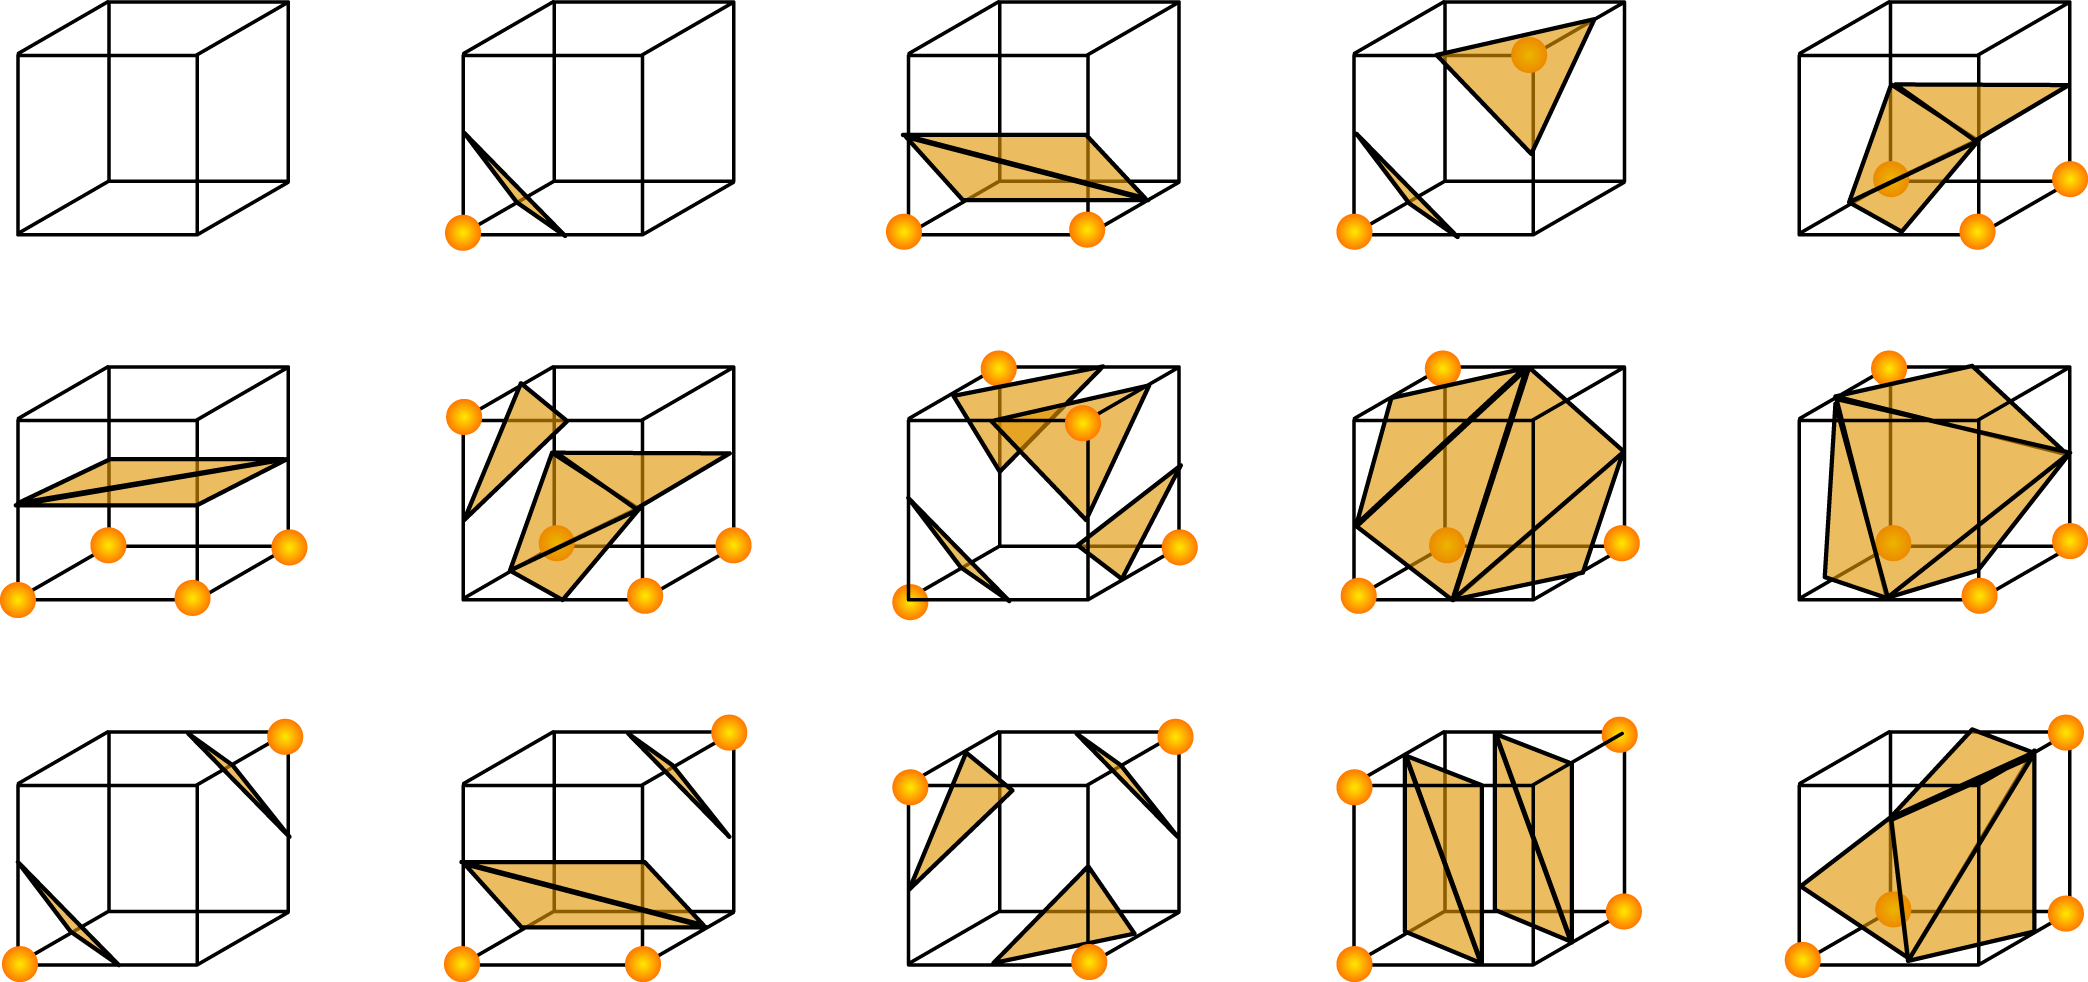
\includegraphics[scale=0.7]{figures/MarchingCubes.png}
    \caption{marching cube算法,图源维基百科\cite{marchingpicture}。首先将空间划分为立方体网格,根据顶点处数值与等值面的关系将立方体分为14种状态。最后根据等值面穿过边的状态生成相应的三角片元。}\label{marching}
\end{figure}
\subsection{评价指标}\label{metric}
为评价重建地图的几何精度,本文使用KD树\cite{kd}(K-Dimension Tree)和KNN\cite{knn}(K-Nearest Neighbors)算法分别从两组顶点数据中计算最邻近点的距离,并使用以下5个指标对重建结果进行评价:距离误差,准确率,召回率,L1倒角距离(Chamfer-L1)和F1-score。进一步,我们将距离误差称为完成度(Completeness),将召回率称为完成率(Completeness Ratio)。

完成度指的是Ground Truth中每个点与其预测结果中的对应点的平均距离。Chamfer-L1距离,也称为曼哈顿倒角距离或L1倒角距离,用于衡量两个集合之间的最短距离。其计算方式是取目标形状的每个边缘点或曲线上的点与参考形状的边缘点或曲线上的点曼哈顿距离后计算平均值或求和。本文设置了一个阈值$threshold$以表示两个点是否重合,若两点距离$d<threshold$,则表示两者重合,即重建成功。使用该方法得出重建结果的准确率与召回率。

具体地说,对于Ground Truth顶点集合与由本文方法重建出的顶点,分别对其进行下采样得到顶点集合$V_{gt}$和$V_{pred}$。接下来对$V_{gt}$中的每一个顶点执行KNN算法,找到其到$V_{pred}$中最近点的距离,得到一个距离集合$D_{r}$。同样的,对$V_{pred}$中的每一个点找到其在$V_{gt}$中距离最近的点,将其距离记录为$D_{p}$。上述各项指标的计算公式如下所示:
\begin{equation*}
\begin{alignedat}{2}
D'_{p} &= \{d \in D_{p} \mid d < threshold\}\;,\\
D'_{r} &= \{d \in D_r\mid d<threshold\}\;,\\
Completeness &= \frac{1}{|D_{r}|}\sum_{i=0}^{|D_{r}|}D_{r}[i]\;\\
Accuracy&= \frac{1}{|D'_{p}|}\sum_{i=0}^{|D'_{p}|}D'_{p}[i]\;,\\
Recall &=\frac{1}{|D'_{r}|}\sum_{i=0}^{|D'_{r}|}D'_{r}[i]\;,\\
Chamfer\_L1 &= \frac{1}{2}\left(Completeness + \frac{1}{|D_{p}|}\sum_{i=0}^{|D_{p}|}D_{p}[i]\right)\;,\\
F1\_score &= \frac{2\times Accuracy\times Recall}{Accuracy + Recall}
\end{alignedat}
\end{equation*}

为评估重建语义建图的精度,本文在数据集点云中进行采样,使用采样点的坐标在完成建图的模型中进行推理得到采样点语义。随后将其与采样点数据集的label进行比较计算得到。本文使用的指标为准确率和交并比,其计算公式为:
\begin{equation*}
    \begin{alignedat}{2}
    \mbox{AUC} &=\quad\;\frac{TP}{TP+FP}\\
    \mbox{IoU} &=\frac{TP}{TP + FP + FN}
    \end{alignedat}
\end{equation*}
\subsection{实验准备}
\subsubsection{数据集}
本文的方法在3个公开的户外激光雷达数据集上进行了定性和定量的测试:(1)人工合成的MaiCity数据集\cite{maicity},模拟使用64线无噪声激光雷达对城市场景扫描序列组成。(2)真实世界的Newer College数据集\cite{ncd},该数据集在牛津大学内使用手持激光雷达记录,具有厘米级测量噪声和大量运动失真。其地面数据使用地面扫描仪获得。两者均带有地面附近的Ground Truth网格数据用作评估。(3) KITTI\cite{KITTI}是目前最大的自动驾驶场景下的计算机视觉算法评测数据集,SemanticKITTI\cite{SemanticKITTI}为其点云数据标注了语义信息。其数据包括激光雷达与RGB-D数据流等,每一帧中出现多个车辆或行人,包含超过20种语义标签类型。
\subsubsection{实验配置}
本文中的两个解码器均为两层全连接层,其中SDF解码器每层有128个节点,语义解码器有256个节点。对于每一帧数据采样1024个点进行训练,设定关键帧窗口大小为5。对于不同的数据集,本文使用表\ref{parameters}中设定的超参数进行训练:
\begin{table}[htbp]
    \centering
    \caption{对于不同数据集,本文方法设定的参数列表}\label{parameters}
    \begin{tabular}[htbp]{llcccc}
        \toprule
        \multicolumn{2}{l}{数据集} & 体素大小(m) & 采样间距(m) & 截断距离(m) &最大碰撞体素数 \\
        \midrule
        \multicolumn{2}{l}{KITTI} & 0.4 & 0.2 &0.3 &20\\
        \multicolumn{2}{l}{Mai City} & 0.2 &0.1&0.2&10\\
        \multicolumn{2}{l}{New College} & 0.4 &0.2&0.3&20\\
        \bottomrule
    \end{tabular}
\end{table}
\subsection{实验结果}
我们进行了是否使用关键帧进行全局建图的对比实验。如图\ref{replay}所示,在左图中我们只使用增量建图线程对KITTI数据集00序列进行建图。地图重建的精细度与准确度随着当前帧位置而变化,即当前帧与当前帧紧邻的帧所影响到的部分场景效果较好。在增量建图线程运行至50帧时,地图右侧新观察到的部分建图效果较好,左侧首先建图的部分已经出现了遗忘问题,地图特征出现缺失,不再连续。当建图线程运行至100帧时,可以看到地图左侧大部分区域的地图细节已经被遗忘,只能解码出大致的轮廓,唯一只有地图右侧正在建图的区域有较好的建图效果。

当使用\ref{forgettingsection}节描述的关键帧选择策略与开启全局建图线程后,如右图所示,即使激光雷达移动至100帧所在位置时,场景中所有已被观察部分的地图特征均被完整保留,遗忘问题得到了明显改善。通过这种方法我们可以降低神经网络的遗忘问题对增量建图的影响。
\begin{figure}[htbp]
	\centering
	\begin{minipage}{0.5\linewidth}
		\centering
		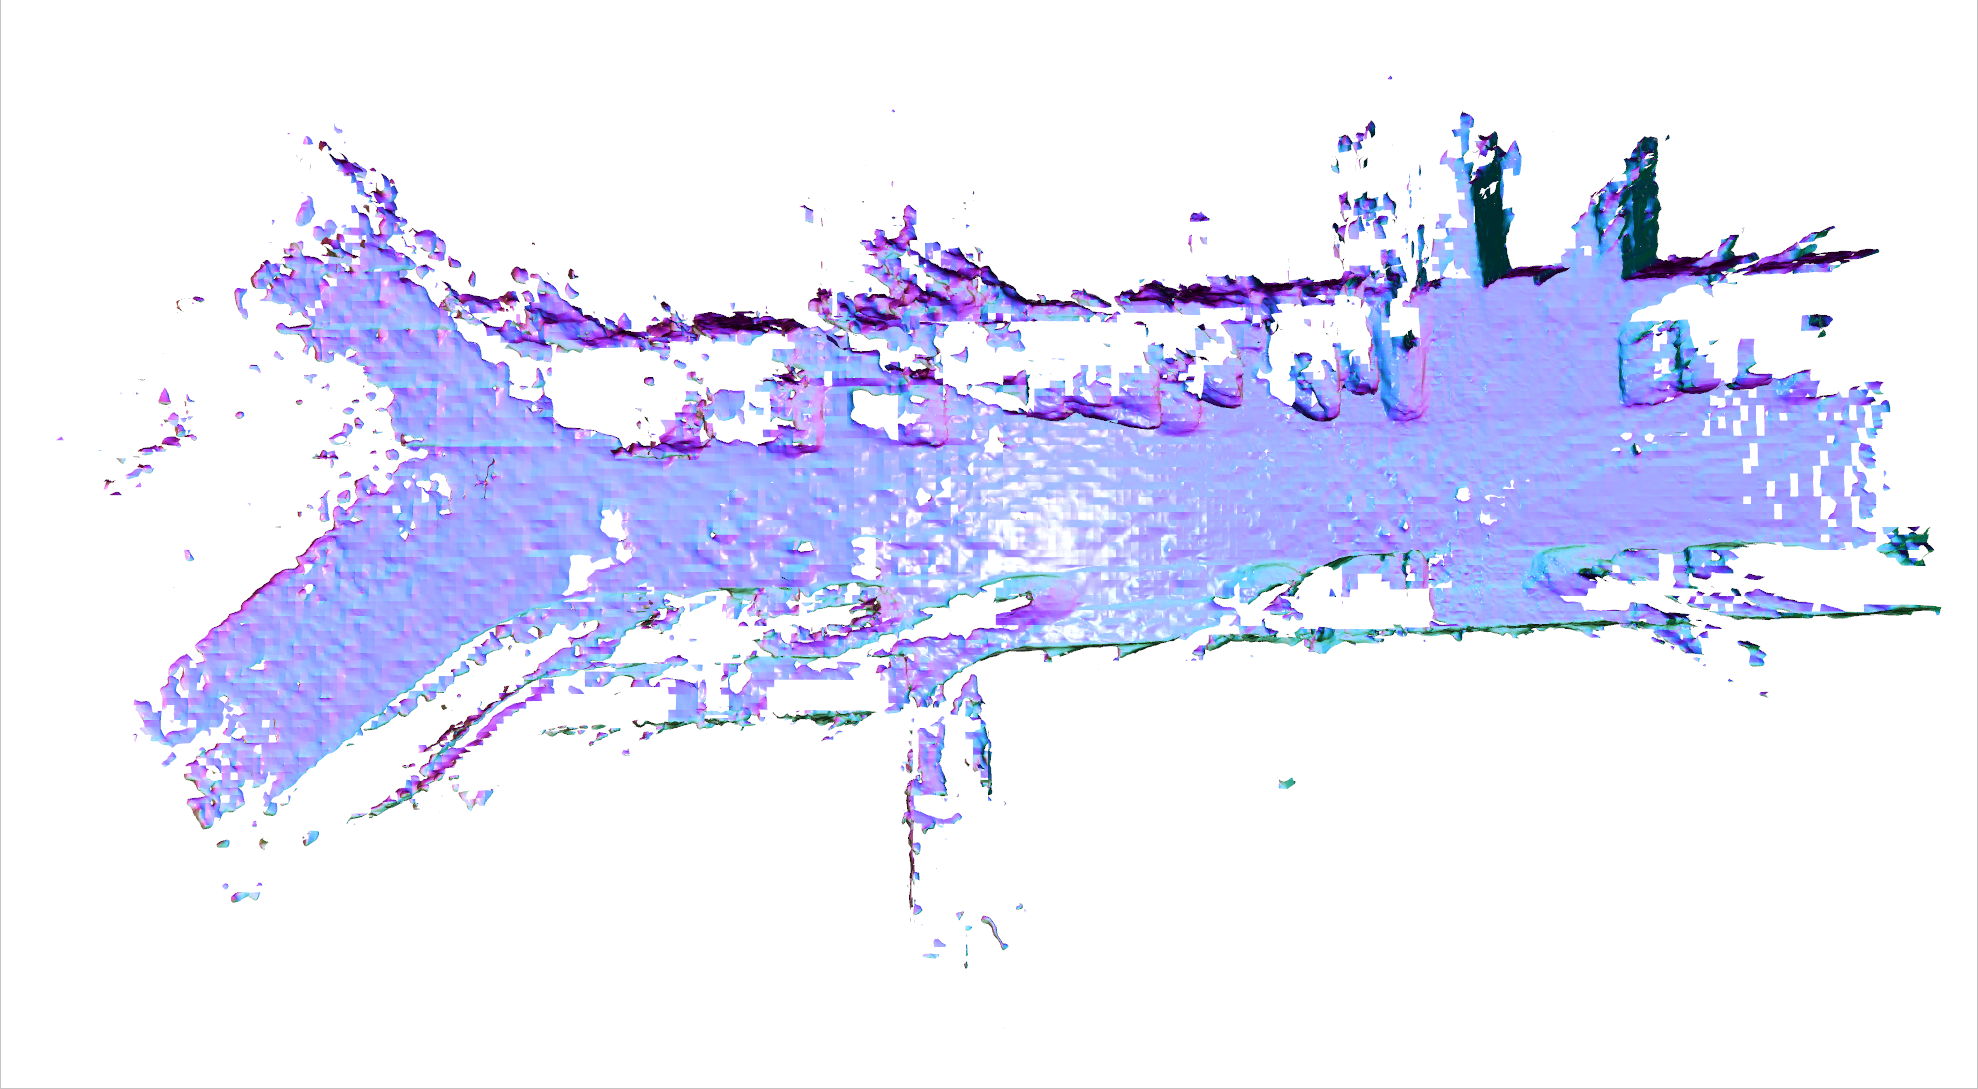
\includegraphics[width=1\linewidth]{figures/50w.png}
        \caption*{不使用replay策略训练50帧}
	\end{minipage}\hfill
	\begin{minipage}{0.5\linewidth}
		\centering
		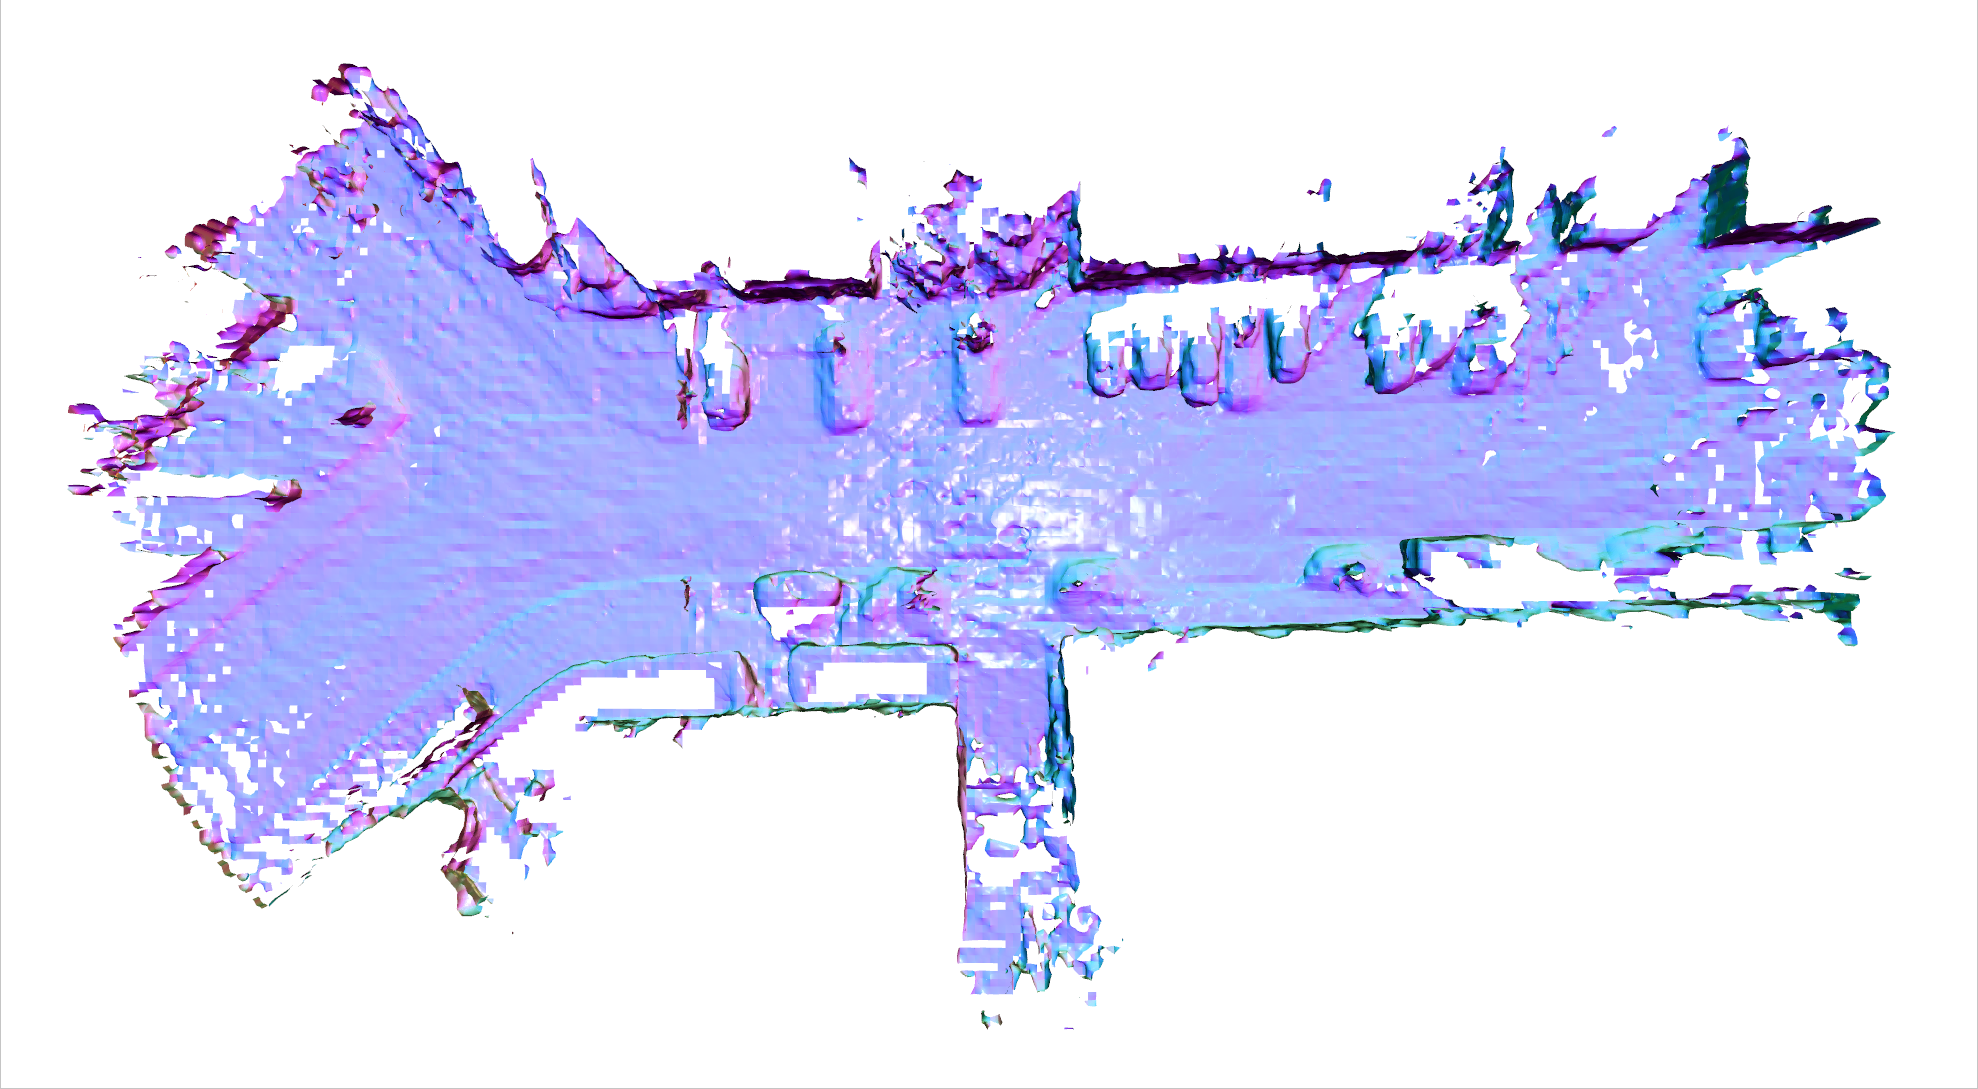
\includegraphics[width=1\linewidth]{figures/50o.png}
        \caption*{使用replay策略训练50帧}
	\end{minipage}
    \vfill
	\begin{minipage}{0.5\linewidth}
		\centering
		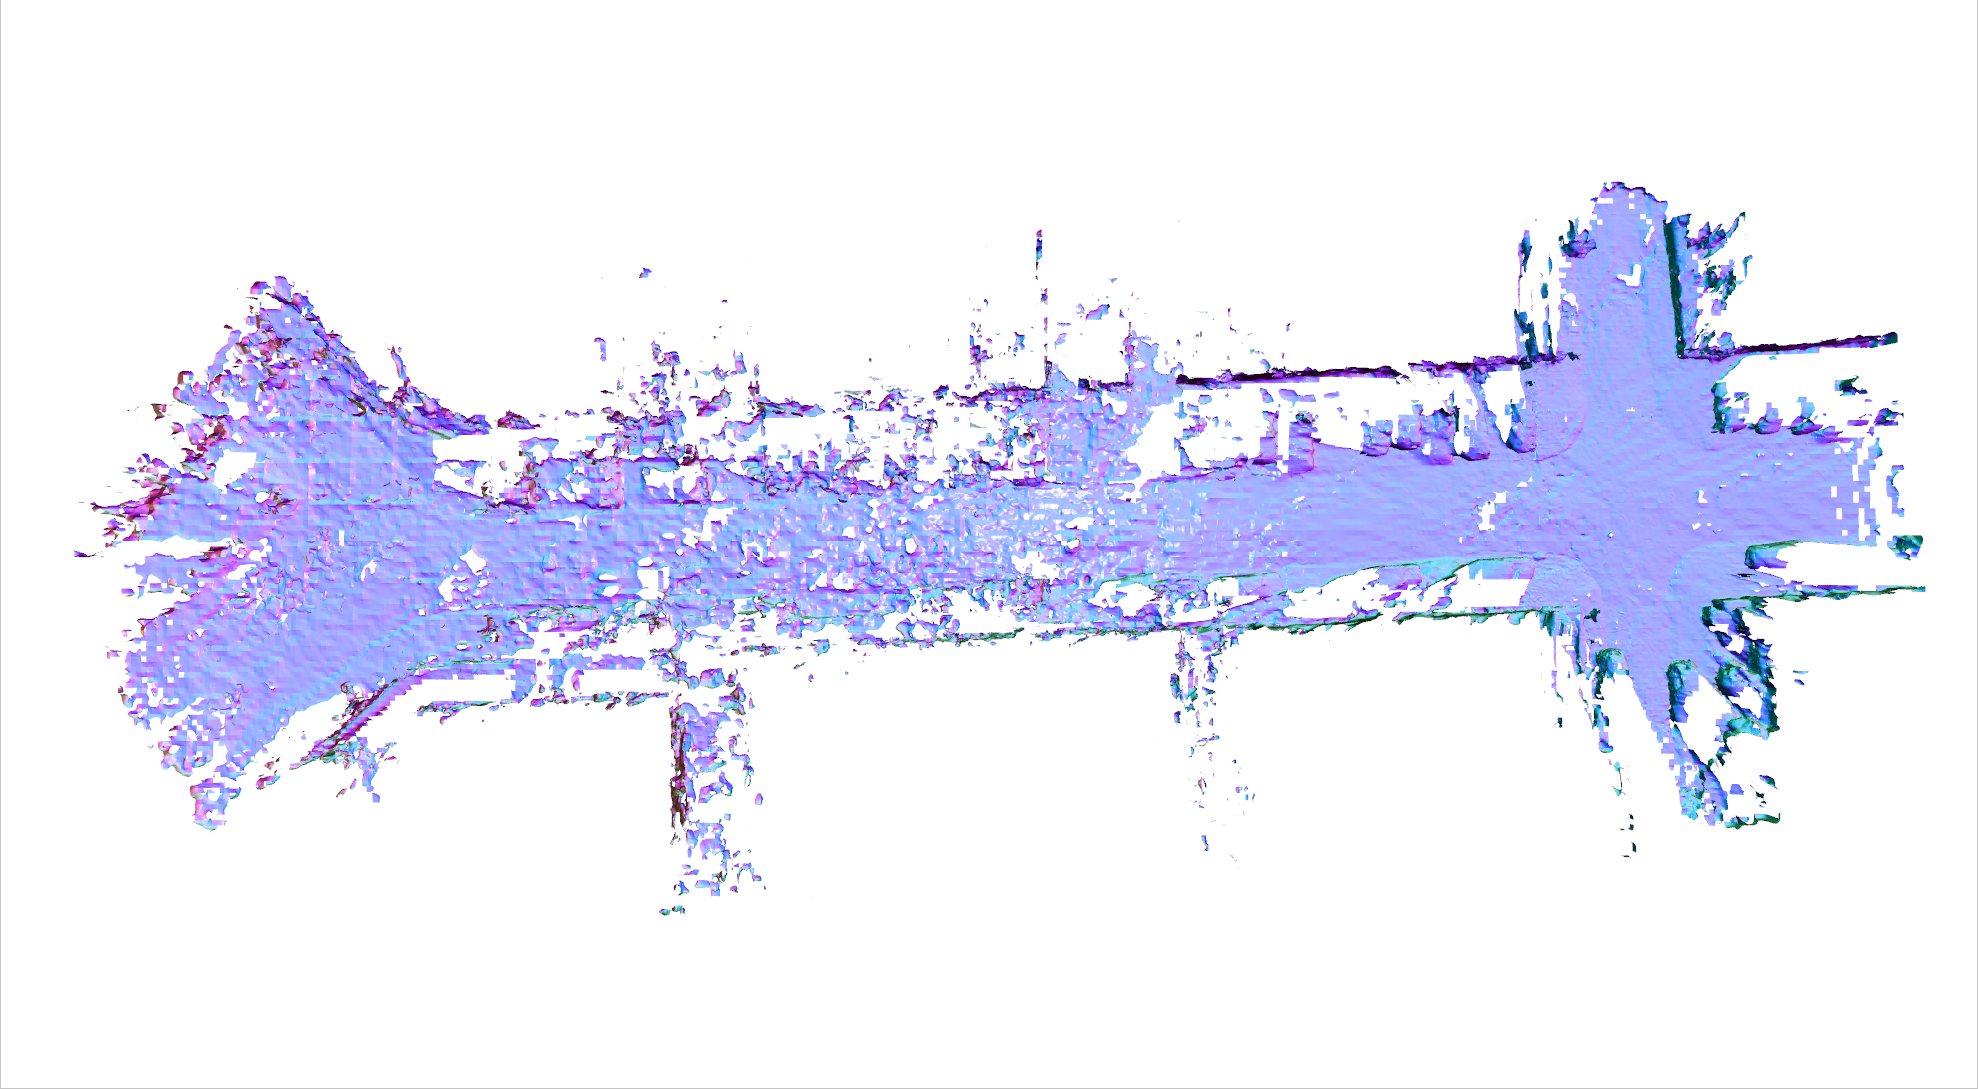
\includegraphics[width=1\linewidth]{figures/100w.png}
        \caption*{不使用replay策略训练100帧}
	\end{minipage}\hfill
	\begin{minipage}{0.5\linewidth}
		\centering
		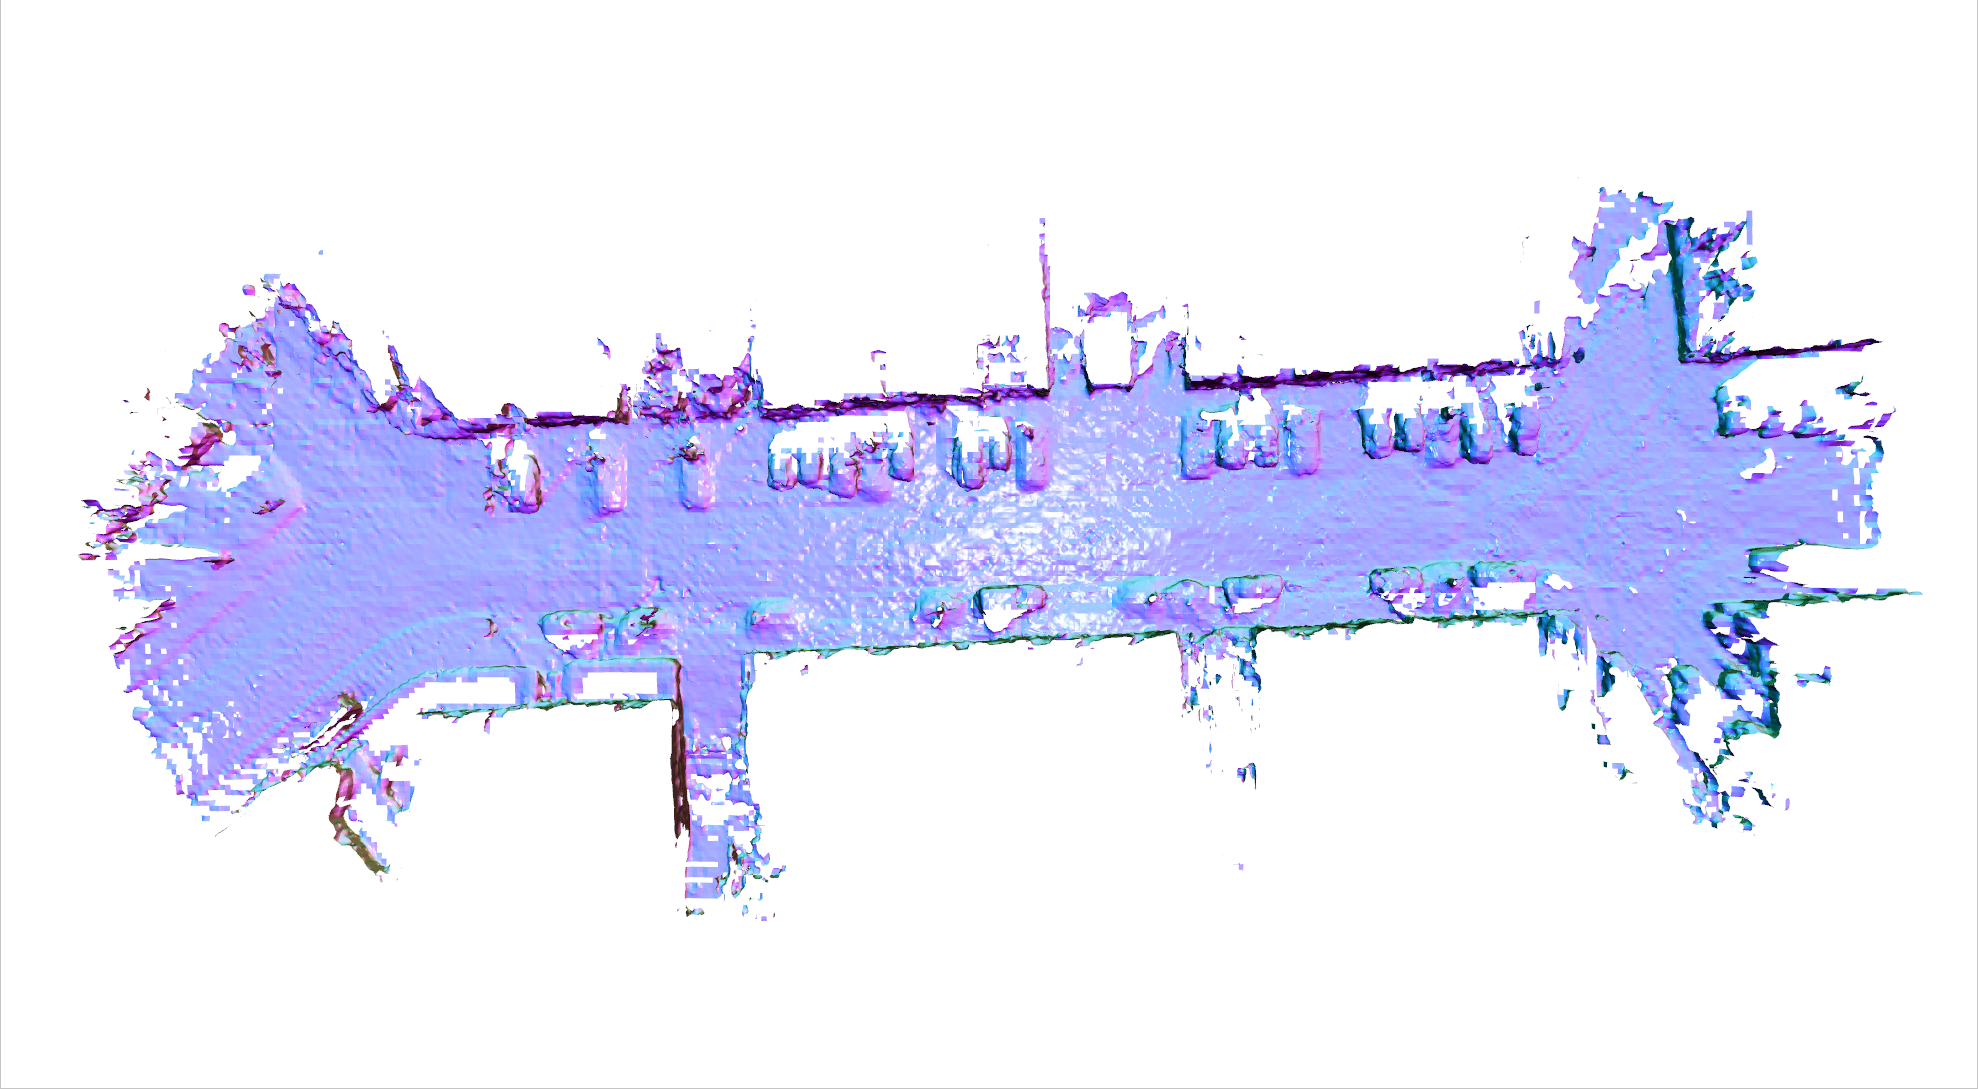
\includegraphics[width=1\linewidth]{figures/100o.png}
        \caption*{使用replay策略训练100帧}
	\end{minipage}
    \caption{在KITTI数据集上是否使用关键帧replay策略的对比实验。在没有使用全局建图线程选择关键帧进行建图的情况下,即使激光雷达只前进50帧时,之前训练的地图部分也会出现遗忘问题。当激光雷达前进100帧时,前50帧所内存的地图信息已经变得非常稀疏。右图使用关键帧选择与全局建图方法后,遗忘问题得到了明显改善,先前的建图准确度与当前帧所在位置无显著联系。}\label{replay}
\end{figure}

同时本文使用式\ref{bce}中的二元交叉熵BCE loss和式\ref{voxloss}中sdf loss与free-space loss结合的方式进行了对比,在KITTI数据集上的结果如图\ref{becornot}所示。在左图中,我们将sdf loss与free-space loss设置相等的权重,结果显示网络并没有准确的学习到场景的表面信息,部分地图区域出现不连续的现象,且地面与墙壁的平滑度没有达到令人满意的程度。在右图中,我们关闭了对前两者损失函数的计算,只采用SDF的二元交叉熵函数对SDF值进行监督,可以看到地图的大部份表面处于连续状态,地面与墙壁等区域较为光滑。这说明网络较好的学习到了SDF值以复原出表面。

基于上述结果,可以得出在监督SDF训练时,使用Sigmoid函数将其映射到[0,1]的区间并使用二元交叉熵损失函数可以使网络更好的学习到场景表面。原因在于Sigmoid函数可以自动的为预测出的SDF值设置截断距离$tr$,以代替sdf loss。并且在物体的表面附近,也就是SDF值期望为0的区域, Sigmoid函数的梯度非常大,使得损失函数输出的结果显著,这也是训练过程中所期望的。
\begin{figure}[htbp]
	\centering
	\begin{minipage}{0.45\linewidth}
		\centering
		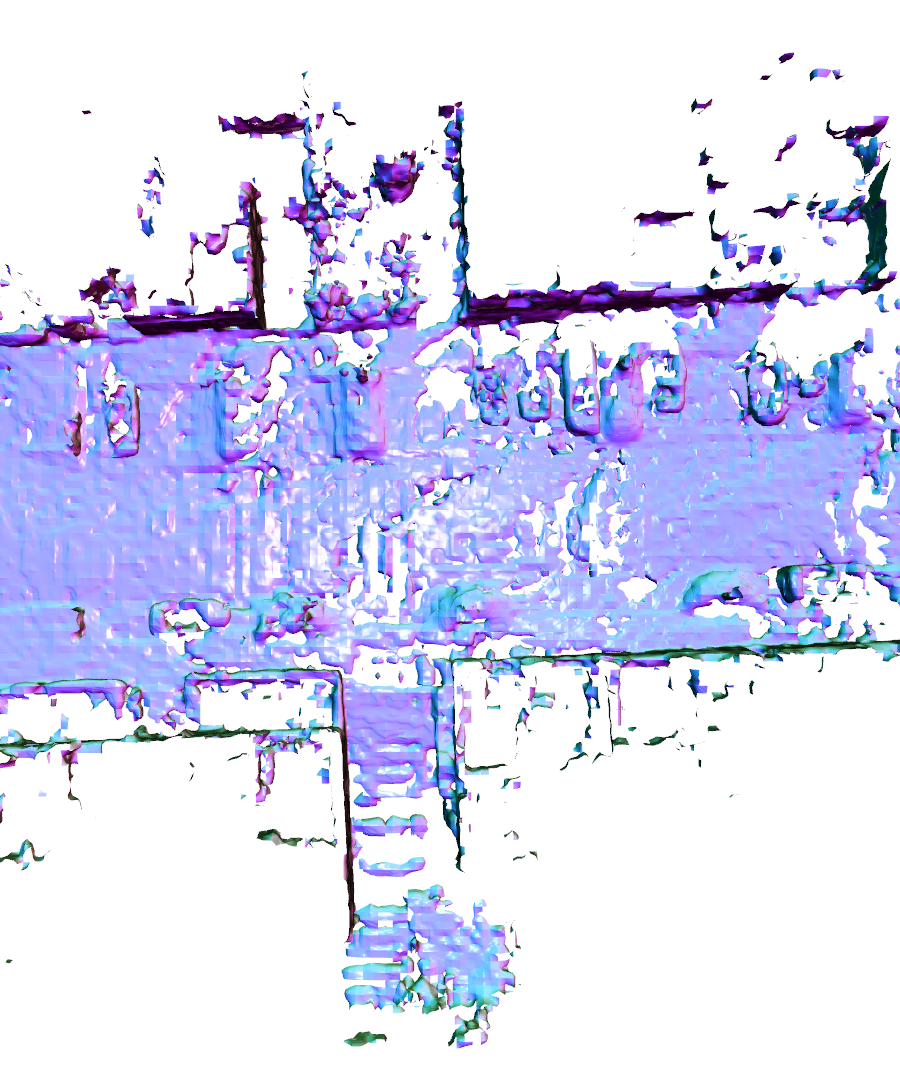
\includegraphics[width=1\linewidth]{figures/kittiwbce.png}
        \caption*{使用sdf loss与free-space loss}
	\end{minipage}
	\begin{minipage}{0.45\linewidth}
		\centering
		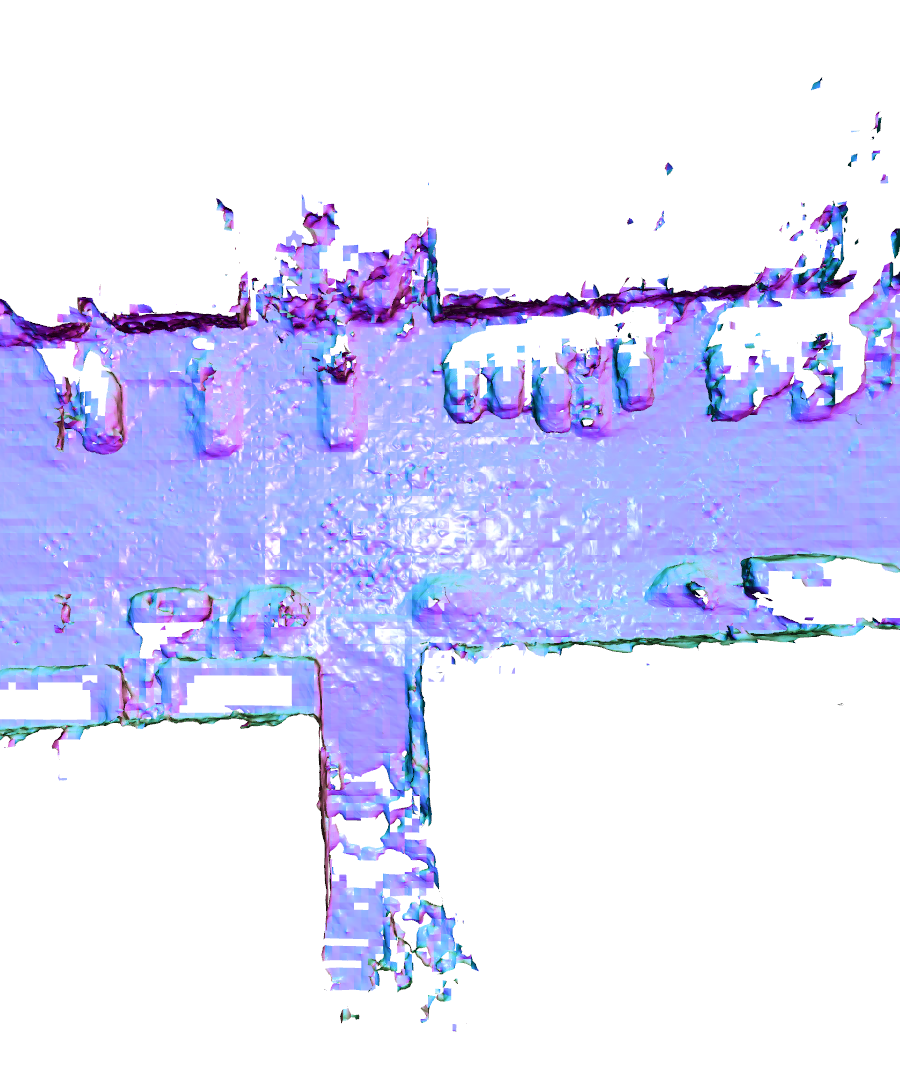
\includegraphics[width=1\linewidth]{figures/kittiobce.png}
        \caption*{使用二元交叉熵BCE loss}
	\end{minipage}
    \caption{在KITTI数据集上使用sdf loss与free-space loss和使用BCE loss的对比实验。左图结果显示特征网络和解码器并未精确学习到地图物体表面,所重建出的场景中地面与墙壁也远远不够平滑。当使用BCE loss对SDF值进行监督训练时,建图效果得到明显改善,如右图所示。}\label{becornot}
\end{figure}
\clearpage
本文使用Voxblox和VDB Fusion,两种基于TSDF的传统视觉SLAM方法与SHINE-Mapping和 Vox-Fusion,两种基于神经隐式表达的建图方法在上述3种数据集上与本文方法进行了比较。除Vox-Fusion外,其余三种方法均可在点云数据集上运行。本文将Vox-Fusion从读取RGB-D数据流扩展至点云数据输入。在3种数据集中, Mai City数据集和New College数据集拥有目标网格的Ground Truth数据,因此可以进行几何精度评估。此外,本文使用SemanticKITTI数据集进行了语义建图的精度评估。本文将实验结果分为无噪声的合成场景与更具挑战性的真实场景进行讨论。
\subsubsection{合成场景}
对于无噪声的合成数据集Mai City,本文使用3种基于神经网络隐式表达的建图方法在Seq01序列上进行实验。如图\ref{mairesult}所示为实验结果。即使在无噪上的场景上,本文方法在细节部分仍优于Vox-Fusion,可以连续的保留车辆轮廓等细节信息。本文使用Mai City的Ground Truth网格数据对几何建图效果进行了评估,结果如表\ref{maicitymetric}所示。在各项指标上,本文方法优于Vox-Fusion。
\begin{figure}[htbp]
    \centering
\begin{minipage}{0.5\linewidth}
    \centering
    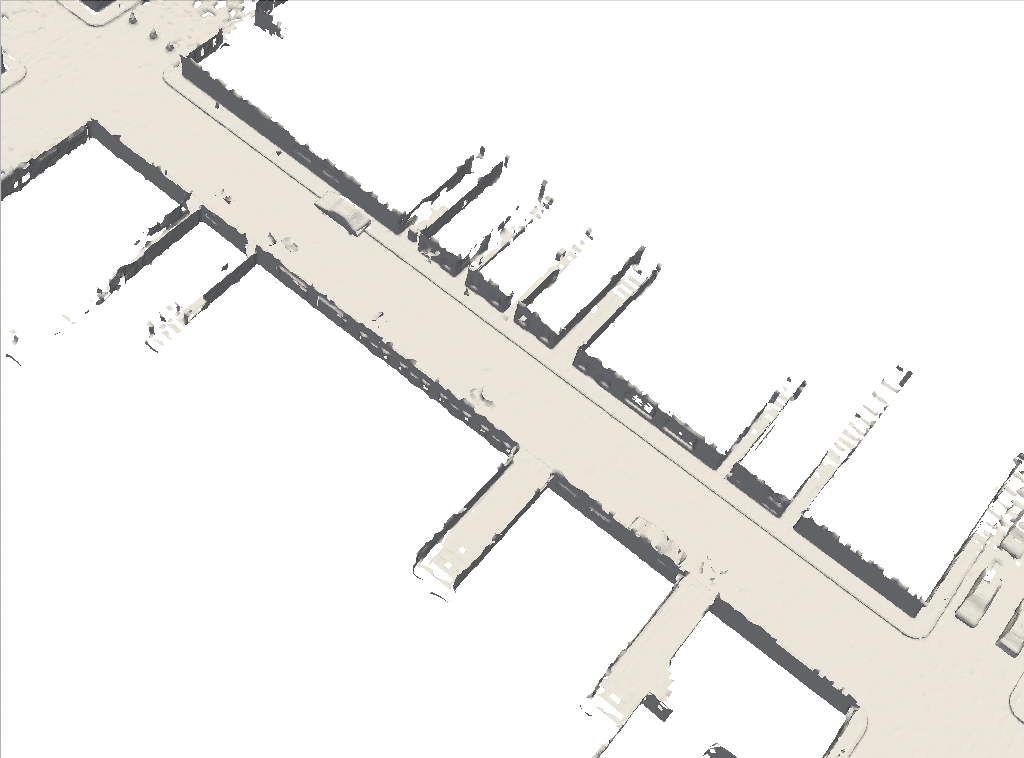
\includegraphics[width=1\linewidth]{figures/mai_3_vox.png}
\end{minipage}\hfill
\begin{minipage}{0.5\linewidth}
    \centering
    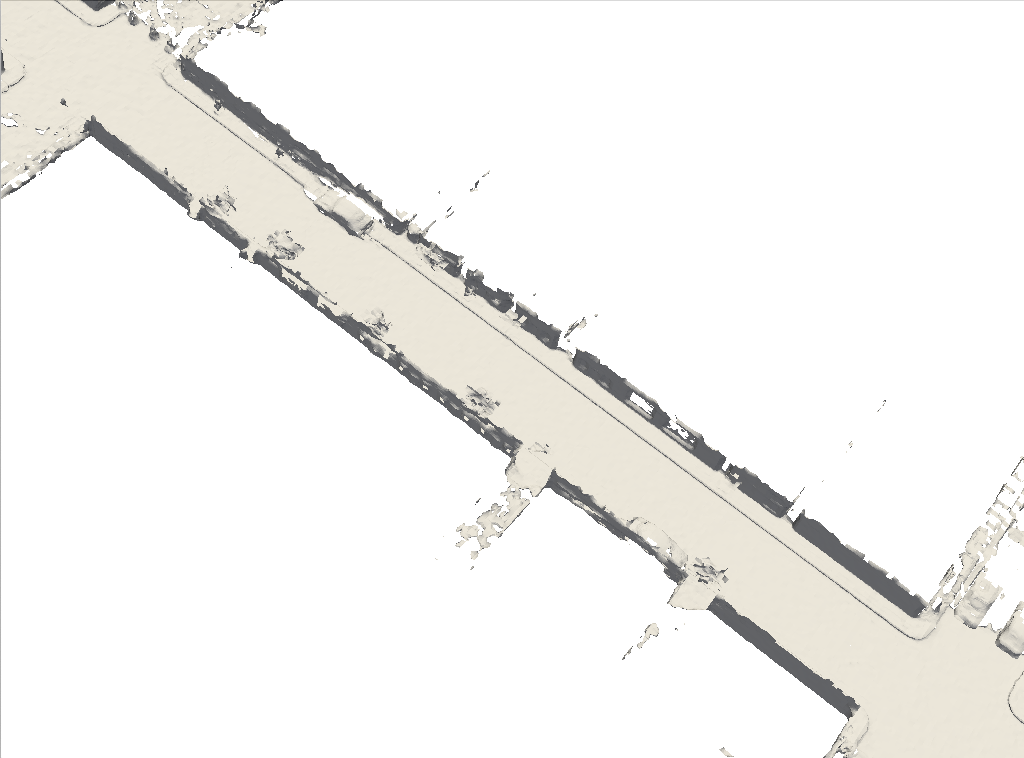
\includegraphics[width=1\linewidth]{figures/mai_3_bce.png}
\end{minipage}
\vfill
\begin{minipage}{0.5\linewidth}
    \centering
    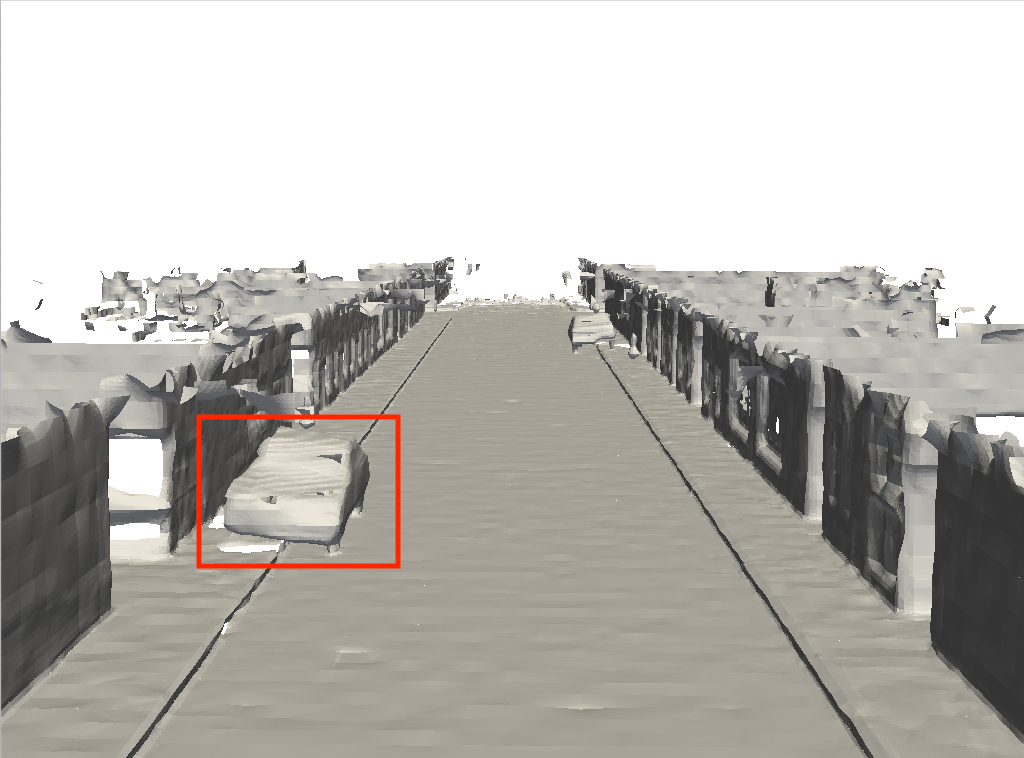
\includegraphics[width=1\linewidth]{figures/mai_1_vox.png}
\end{minipage}\hfill
\begin{minipage}{0.5\linewidth}
    \centering
    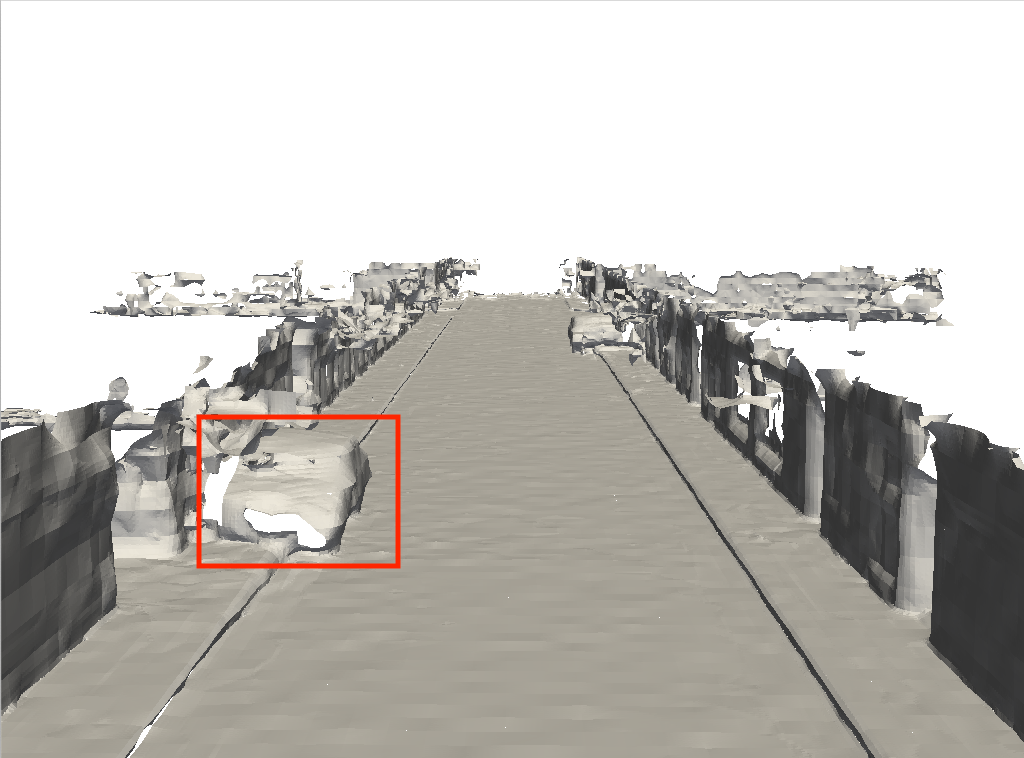
\includegraphics[width=1\linewidth]{figures/mai_1_bce.png}
\end{minipage}
\vfill
\begin{minipage}{0.5\linewidth}
    \centering
    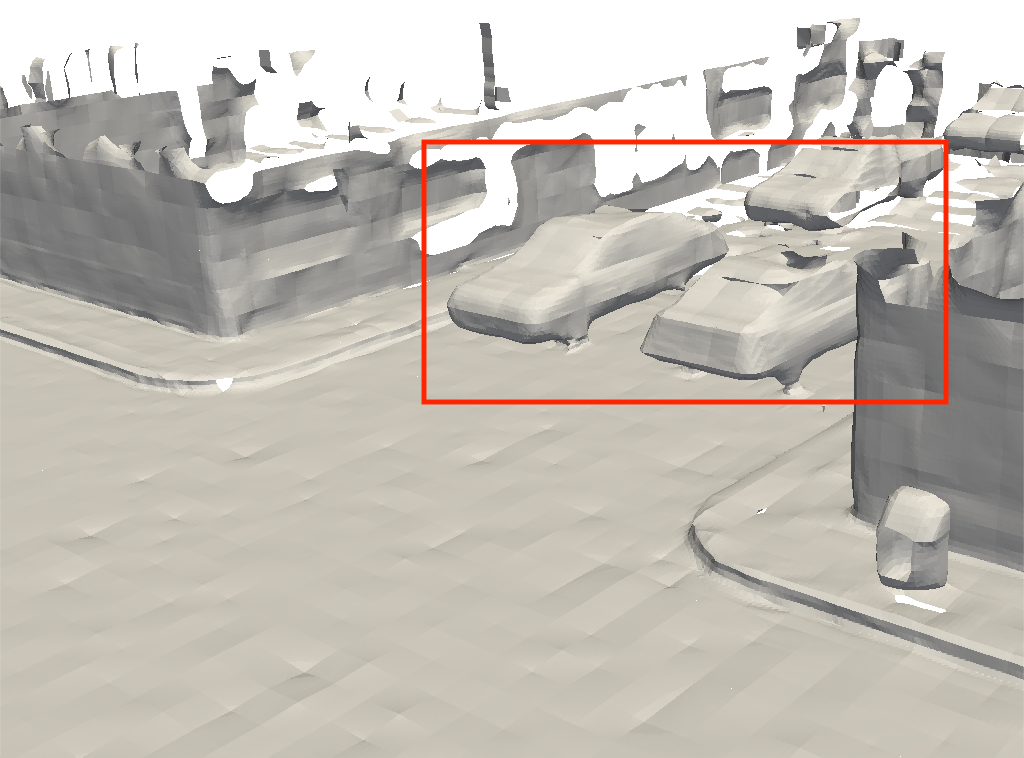
\includegraphics[width=1\linewidth]{figures/mai_2_vox.png}
    \caption*{(a)Ours}
\end{minipage}\hfill
\begin{minipage}{0.5\linewidth}
    \centering
    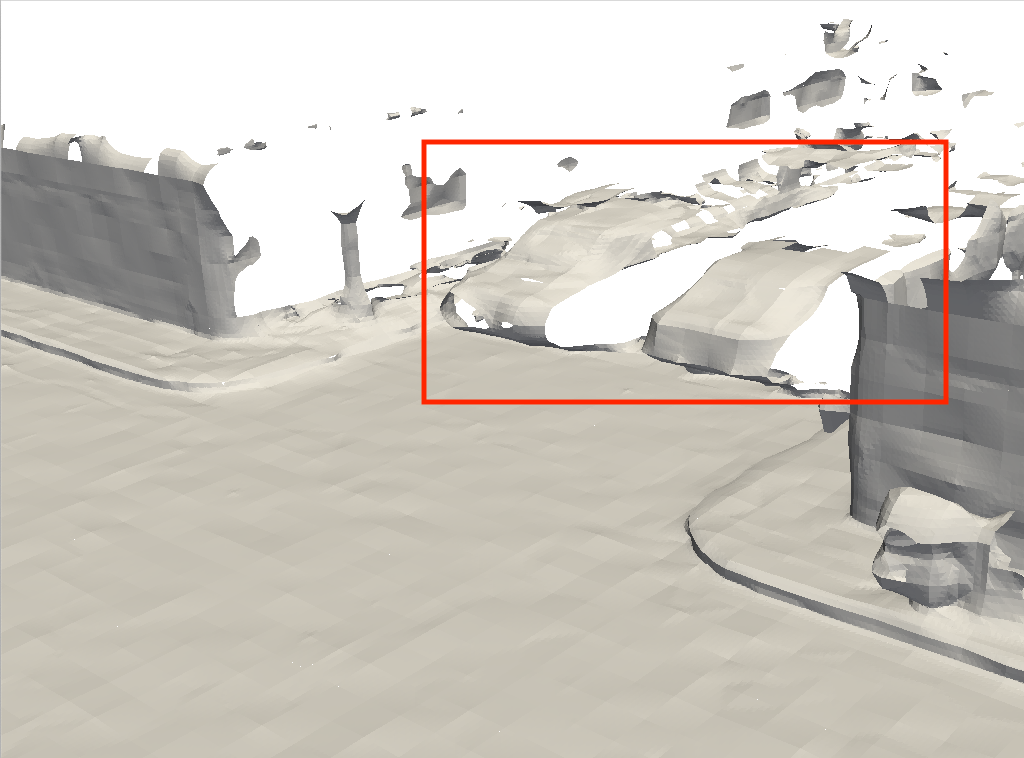
\includegraphics[width=1\linewidth]{figures/mai_2_bce.png}
    \caption*{(b)Vox-Fusion}
\end{minipage}
\end{figure}

\begin{figure}[htbp]
    \centering
    \begin{minipage}{0.5\linewidth}
    \centering
    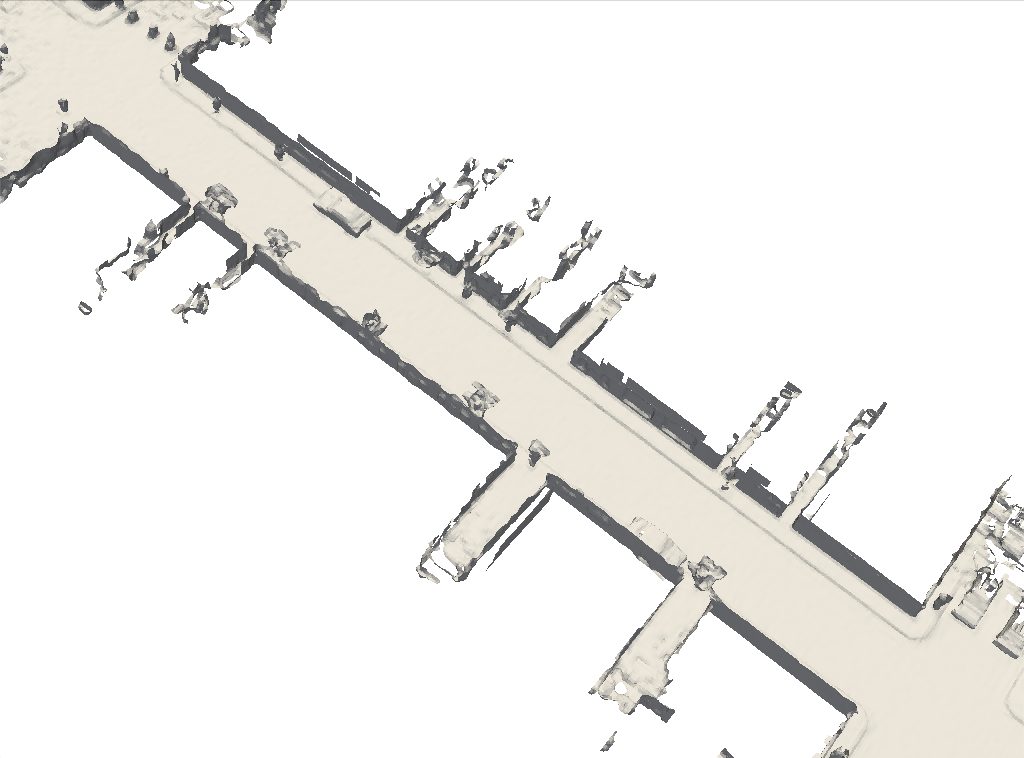
\includegraphics[width=1\linewidth]{figures/mai_3_shine.png}
    \end{minipage}\hfill
    \begin{minipage}{0.5\linewidth}
    \centering
    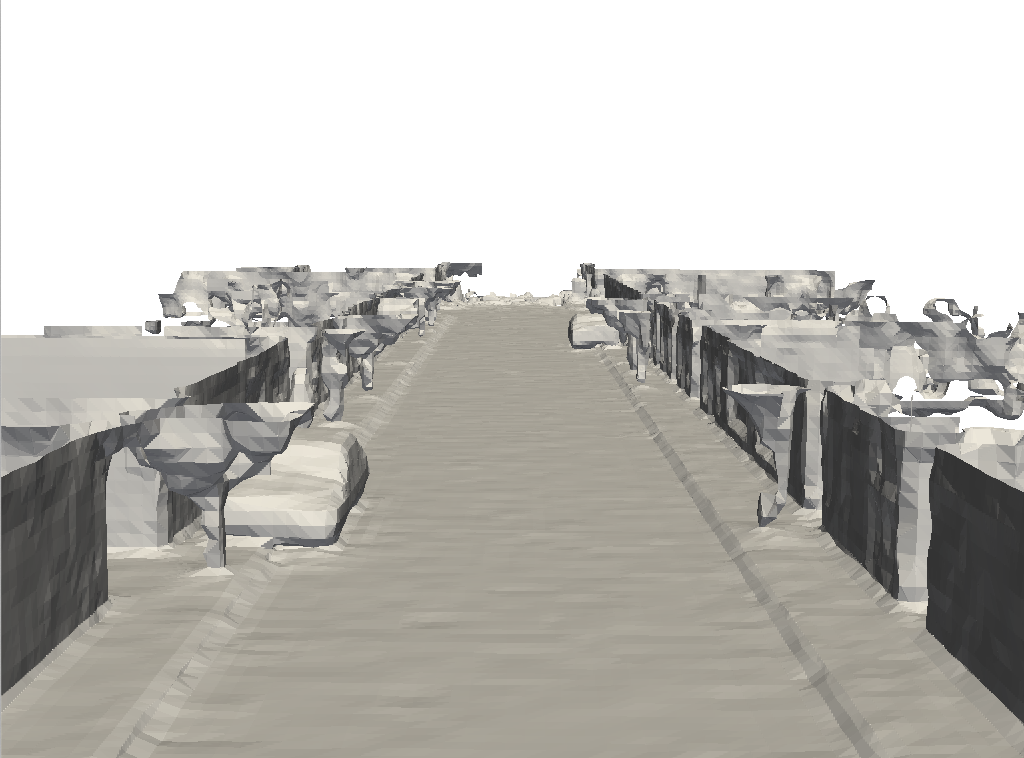
\includegraphics[width=1\linewidth]{figures/mai_1_shine.png}
    \end{minipage}
    \vfill
    \begin{minipage}{0.5\linewidth}
    \centering
    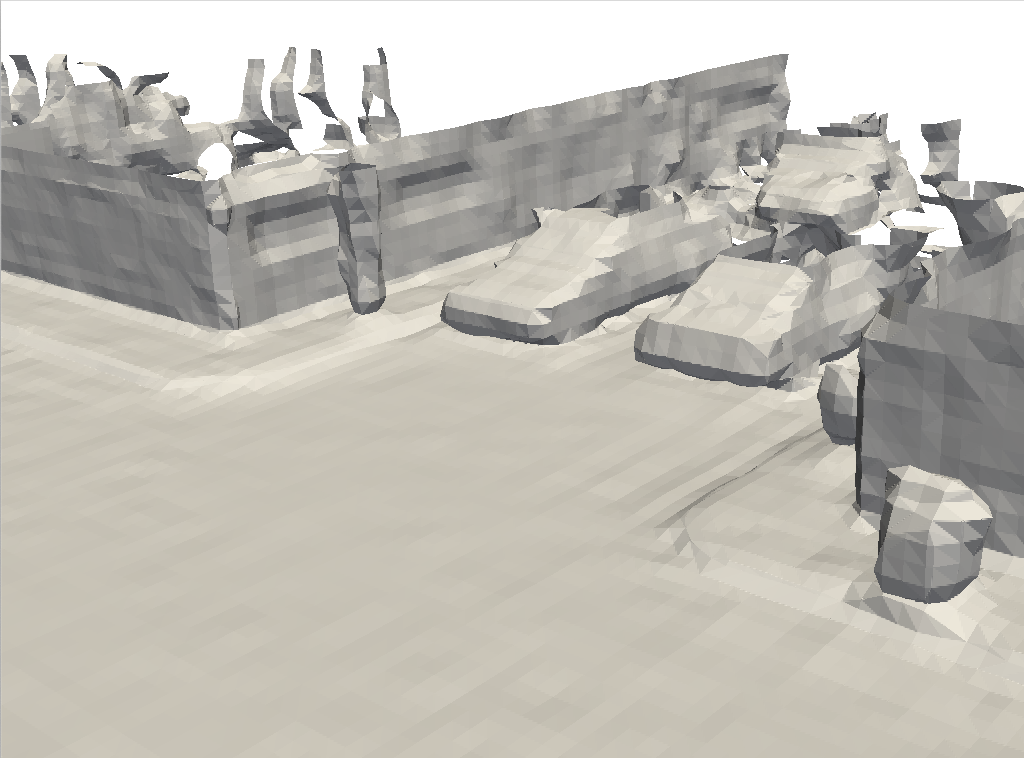
\includegraphics[width=1\linewidth]{figures/mai_2_shine.png}
    \end{minipage}\caption*{(c)SHING-Mapping}
    \caption{3种基于神经网络的隐式建图方法在Mai City数据集上的结果。}\label{mairesult}
\end{figure}
\begin{table}[htbp]
    \centering
    \caption{定性测量的不同方法在Mai City数据集上建图的几何精度,将目标地图与重建地图之间对应点重合的阈值$threshold$设置为10cm。}\label{maicitymetric}
    \begin{tabular}[htbp]{llccccc}
        \toprule
        \multicolumn{2}{l}{方法} & $\mathbf{Comp.}$(cm) & $\mathbf{Acc.}(\%)$ & $\mathbf{C-l1}$(cm) &  $\mathbf{Comp. Ratio}$(\%) &$\mathbf{F1-score}$\\
        \midrule
        \multicolumn{2}{l}{Voxblox} & 7.1 & 93.3 & 4.8 &84.0&90.0\\
        \multicolumn{2}{l}{VDB Fusion} & 6.9&92.1&4.5&90.2&94.1 \\
        \multicolumn{2}{l}{SHINE-Mapping} & 3.2&94,6&2.9&95.2&95.9 \\
        \multicolumn{2}{l}{Vox-Fusion} & 18.0 & 90.3 &11.2&76.3&82.8\\
        \midrule
        \multicolumn{2}{l}{Ours+bce} & 12.5&95.2 &8.3&85.7&90.2\\
        \bottomrule
    \end{tabular}
\end{table}
\subsubsection{真实场景}
本文使用5种方法在KITTI数据集Seq00序列的前200帧上进行建图。实验结果如图\ref{kittiresult}所示。可以看到本文方法在建图效果上媲美SHINE-Mapping与VDB Fusion,以相同的建图速度和更低的分辨率达到了相同的效果。本文使用的优化方法在地图细节处理上效果优于Vox-Fusion,如车辆,墙壁等细节。实验证明本文方法可以在真实数据集上对室外大规模地图进行实时建图,在保留细节的同时保持地图的连续性。
\begin{figure}[htbp]
	\centering
	\begin{minipage}{0.5\linewidth}
		\centering
		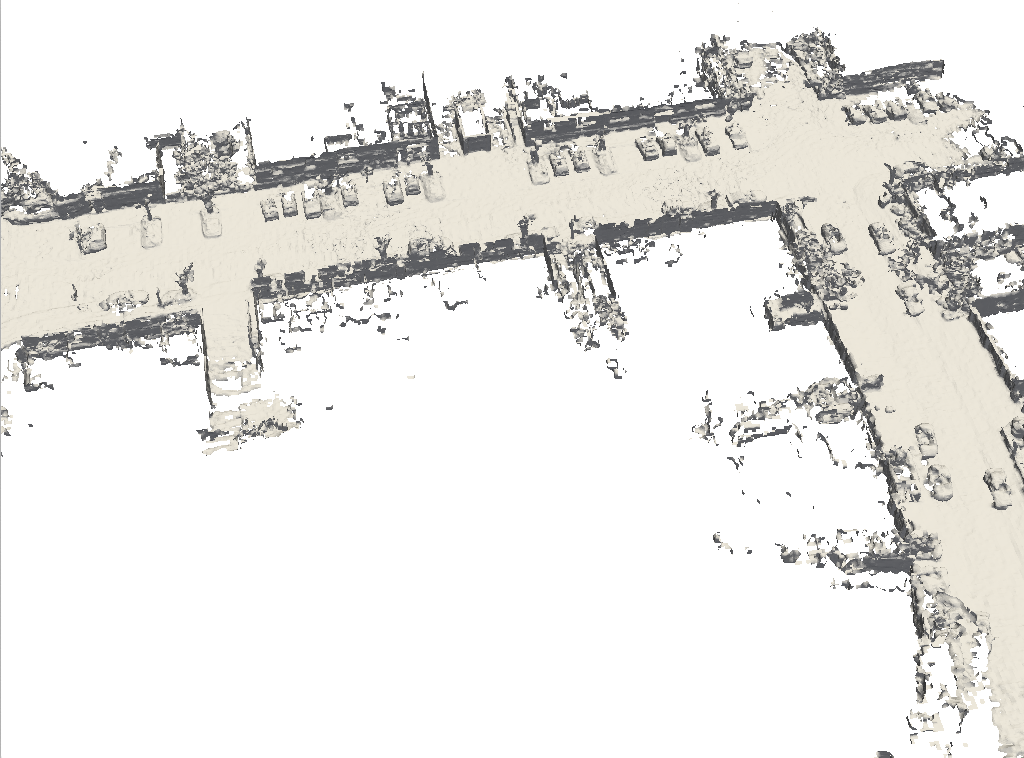
\includegraphics[width=1\linewidth]{figures/kitti_1_vox.png}
	\end{minipage}\hfill
	\begin{minipage}{0.5\linewidth}
		\centering
		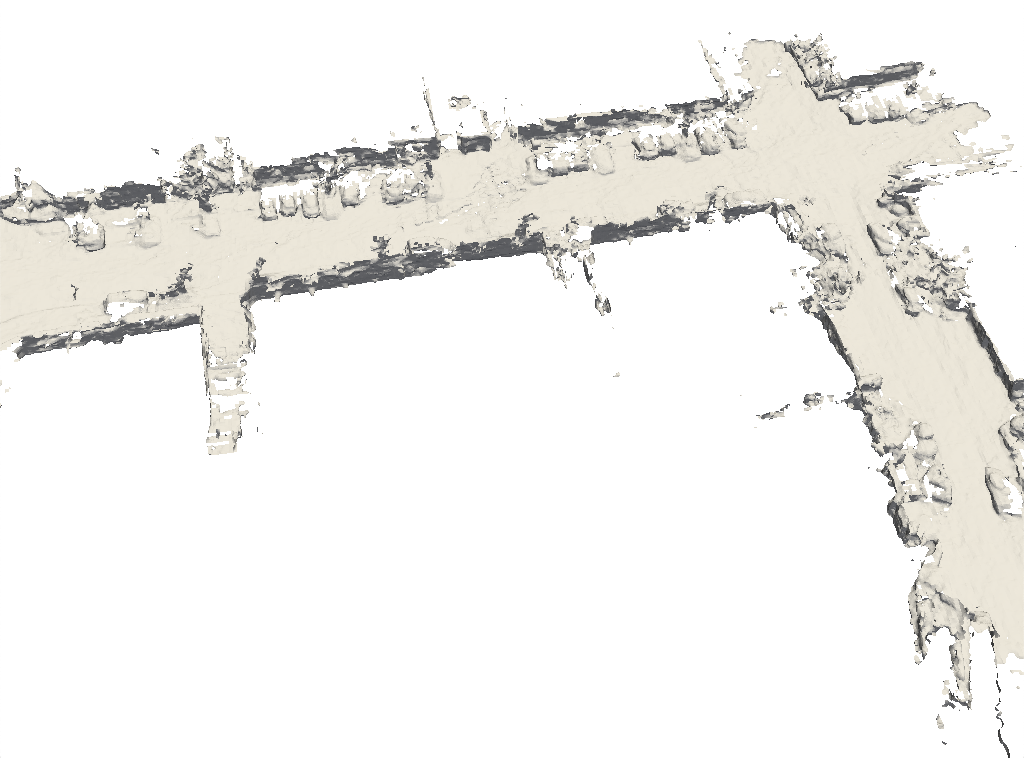
\includegraphics[width=1\linewidth]{figures/kitti_1_bce.png}
	\end{minipage}
    \vfill
    \begin{minipage}{0.5\linewidth}
		\centering
		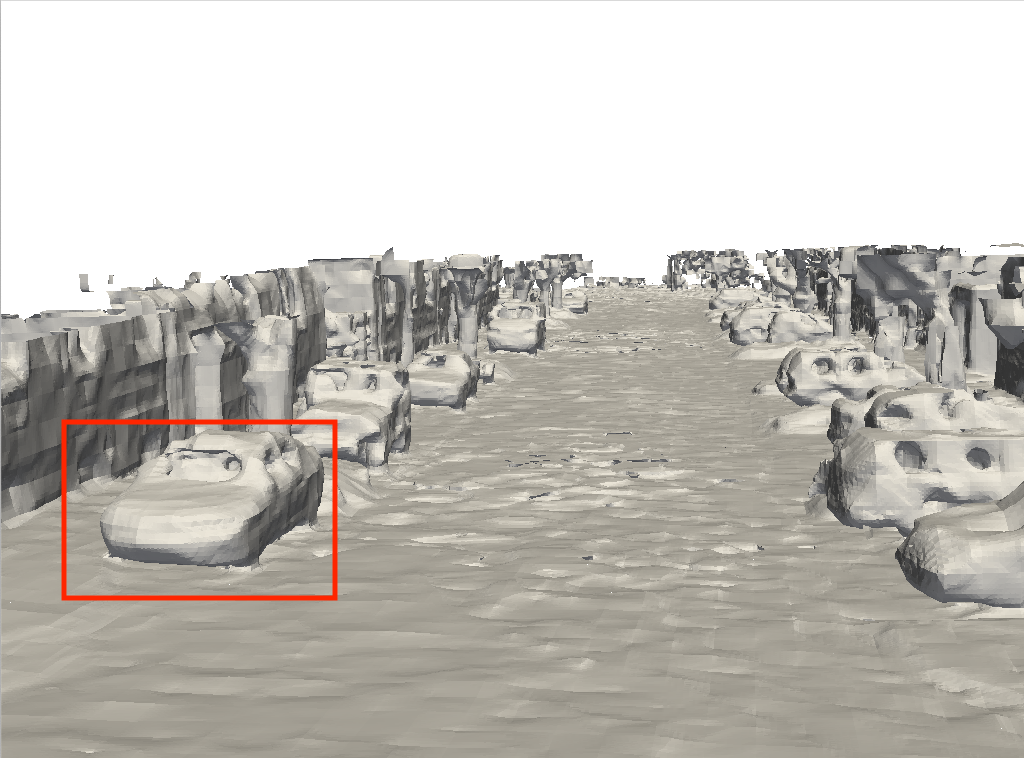
\includegraphics[width=1\linewidth]{figures/kitti_2_vox.png}
	\end{minipage}\hfill
	\begin{minipage}{0.5\linewidth}
		\centering
		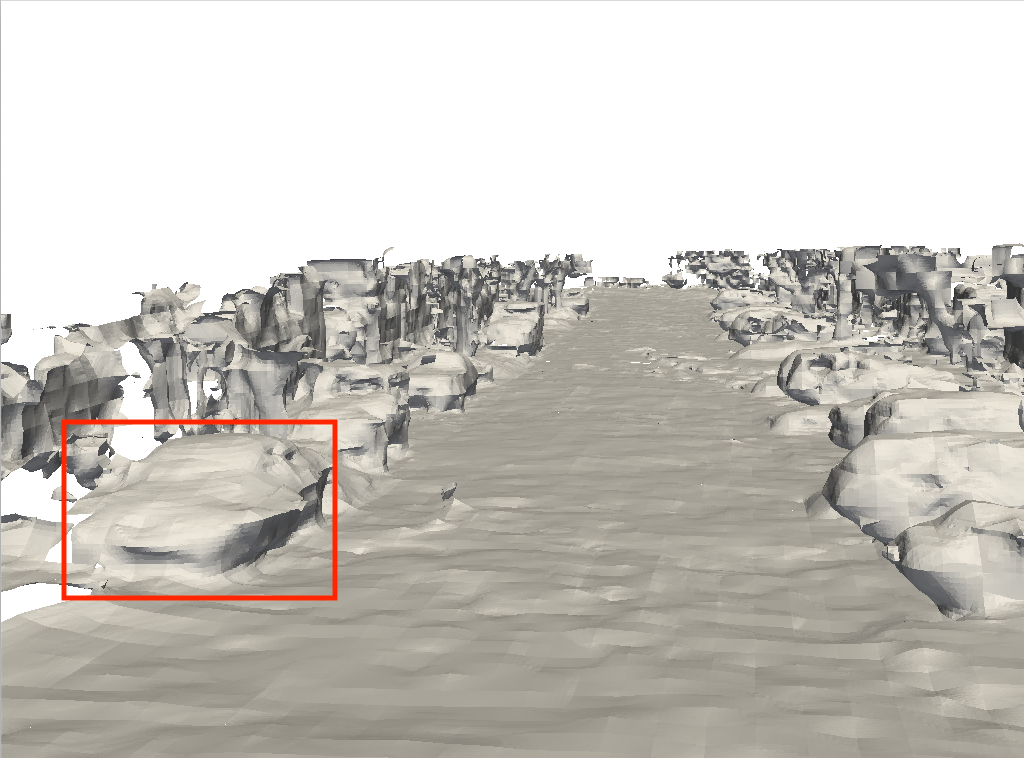
\includegraphics[width=1\linewidth]{figures/kitti_2_bce.png}
	\end{minipage}
    \vfill
	\begin{minipage}{0.5\linewidth}
		\centering
		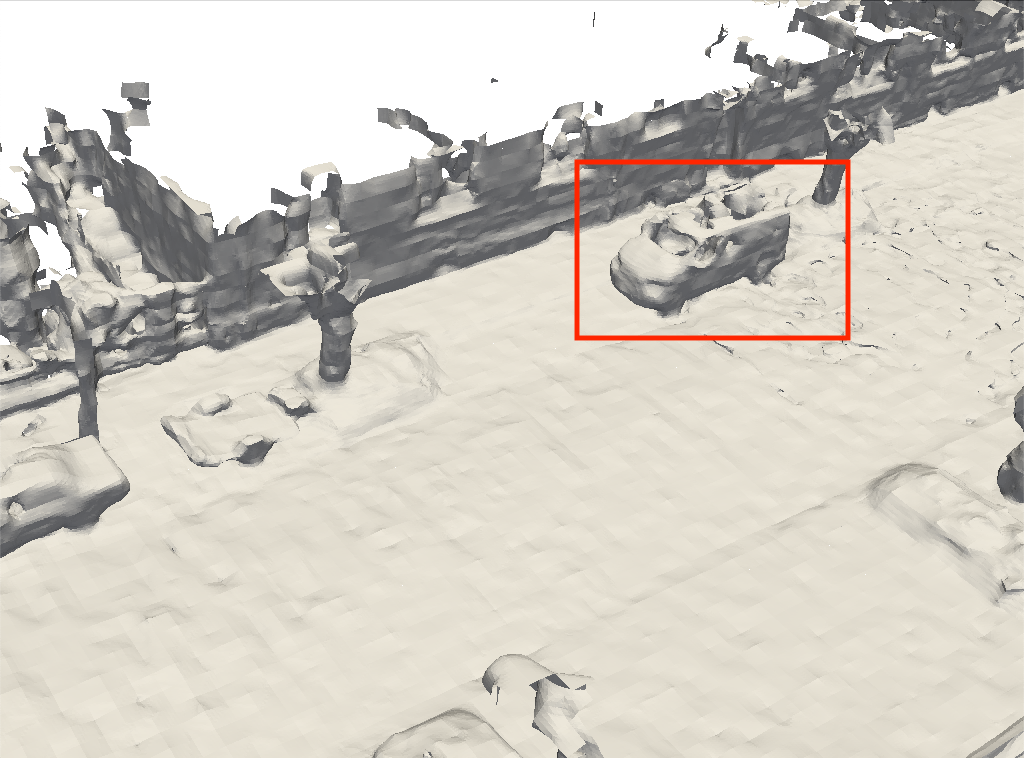
\includegraphics[width=1\linewidth]{figures/kitti_3_vox.png}
        \caption*{(a)Ours}
	\end{minipage}\hfill
    \begin{minipage}{0.5\linewidth}
		\centering
		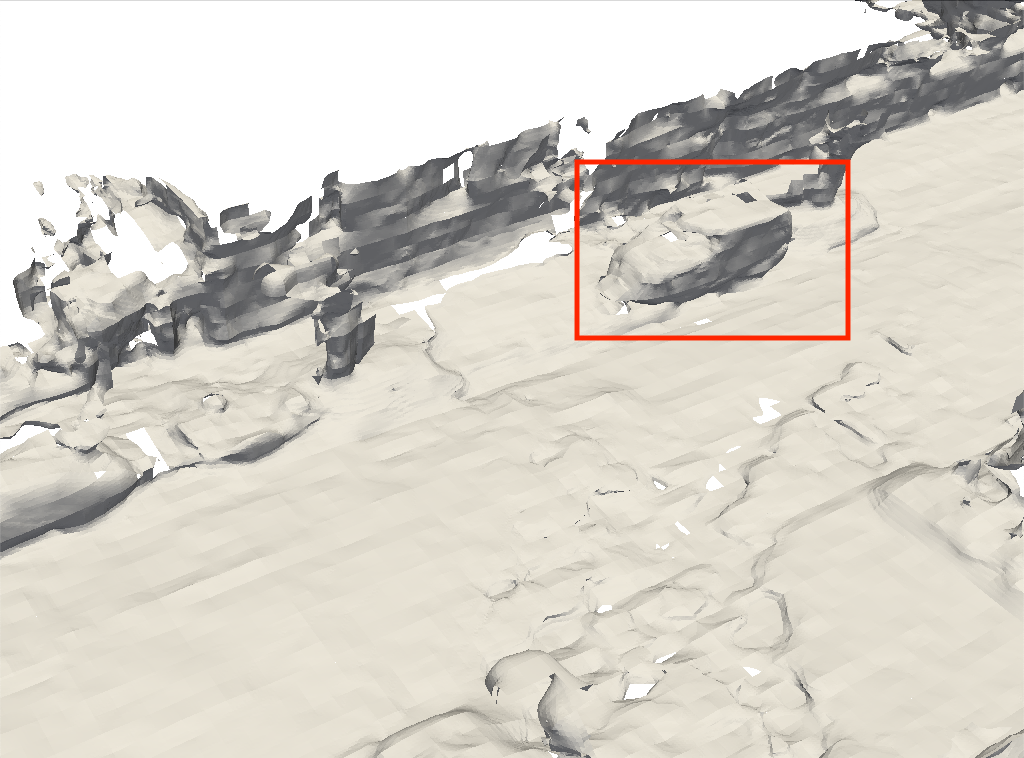
\includegraphics[width=1\linewidth]{figures/kitti_3_bce.png}
        \caption*{(b)Vox-Fusion}
	\end{minipage}
\end{figure}
\begin{figure}[htbp]
        \centering
    \begin{minipage}{0.5\linewidth}
		\centering
		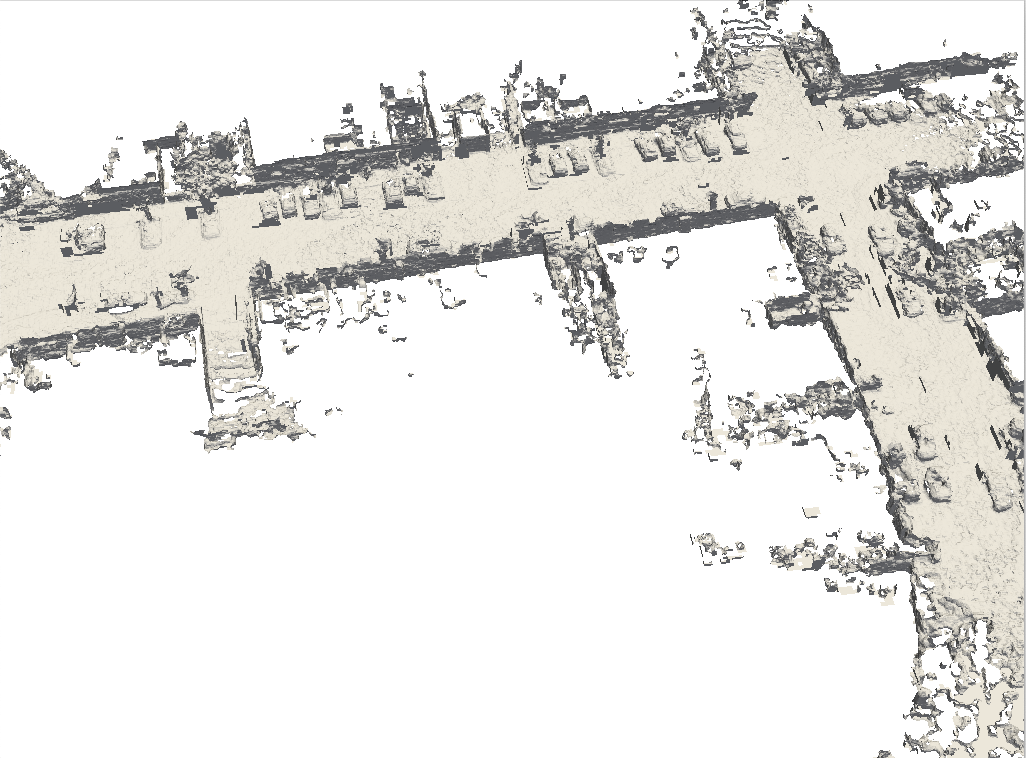
\includegraphics[width=1\linewidth]{figures/kitti_1_shine.png}
	\end{minipage}\hfill
	\begin{minipage}{0.5\linewidth}
		\centering
		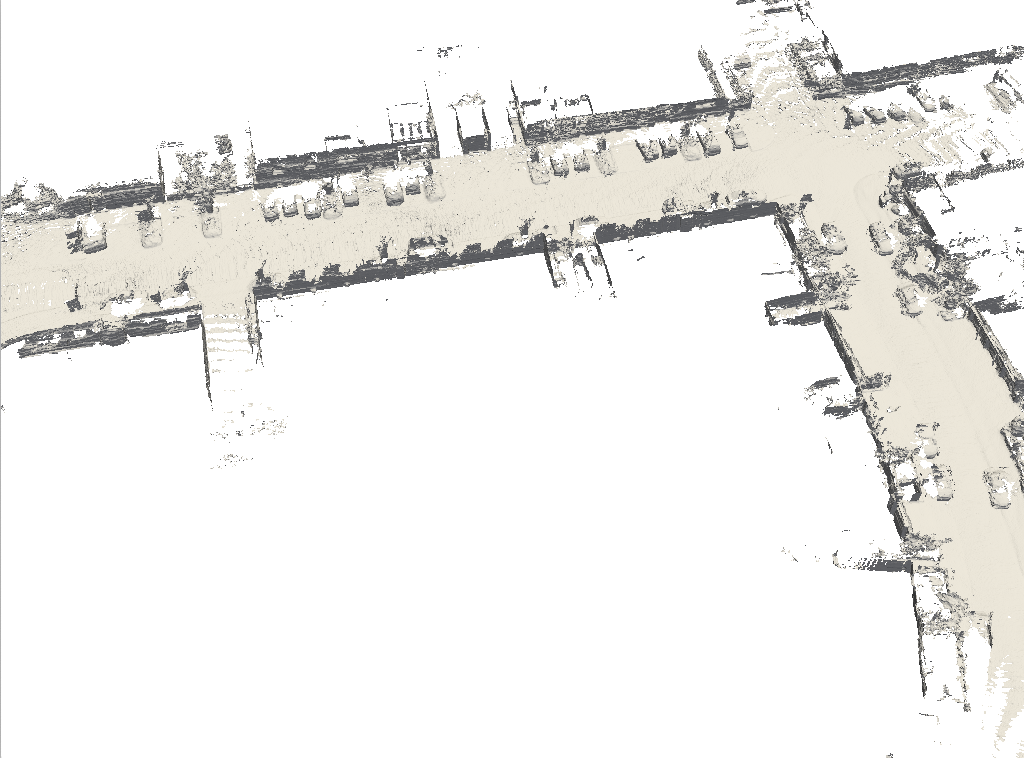
\includegraphics[width=1\linewidth]{figures/kitti_1_vdb.png}
	\end{minipage}
    \vfill
    \begin{minipage}{0.5\linewidth}
		\centering
		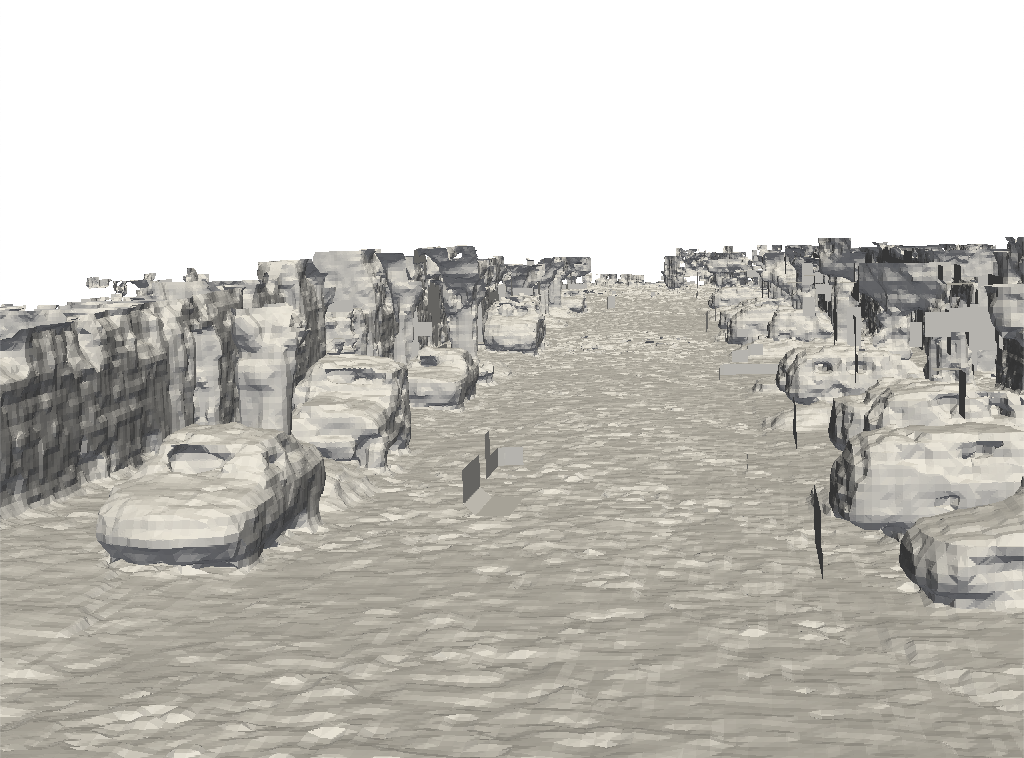
\includegraphics[width=1\linewidth]{figures/kitti_2_shine.png}
	\end{minipage}\hfill
	\begin{minipage}{0.5\linewidth}
		\centering
		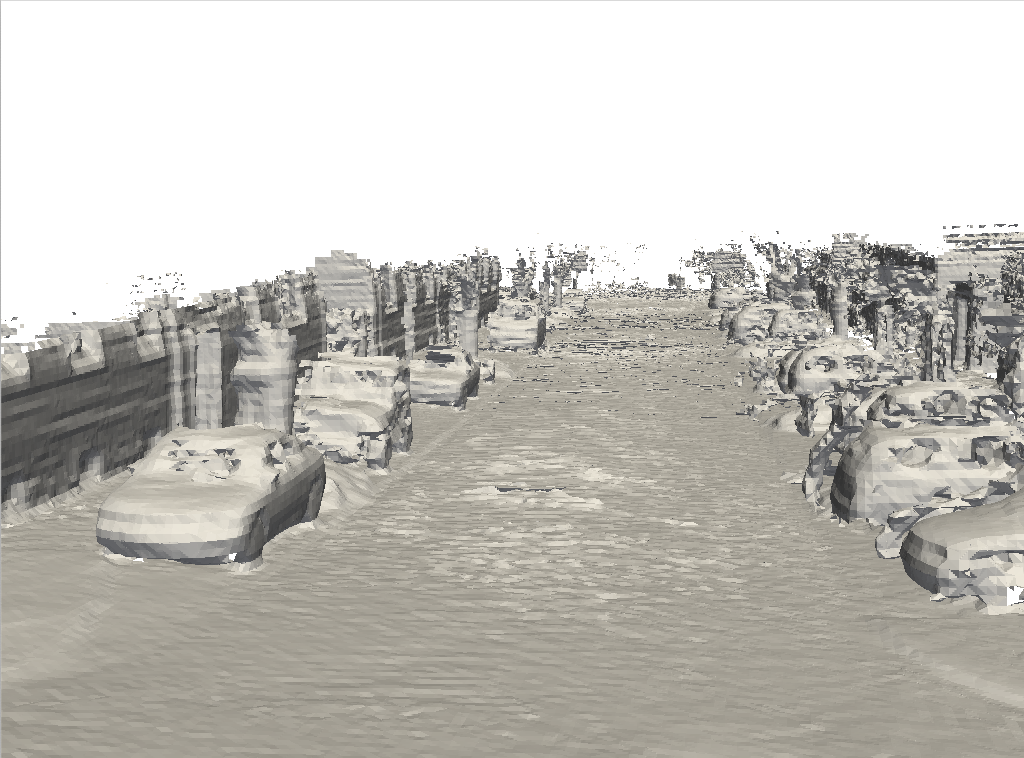
\includegraphics[width=1\linewidth]{figures/kitti_2_vdb.png}
	\end{minipage}
    \vfill
	\begin{minipage}{0.5\linewidth}
		\centering
		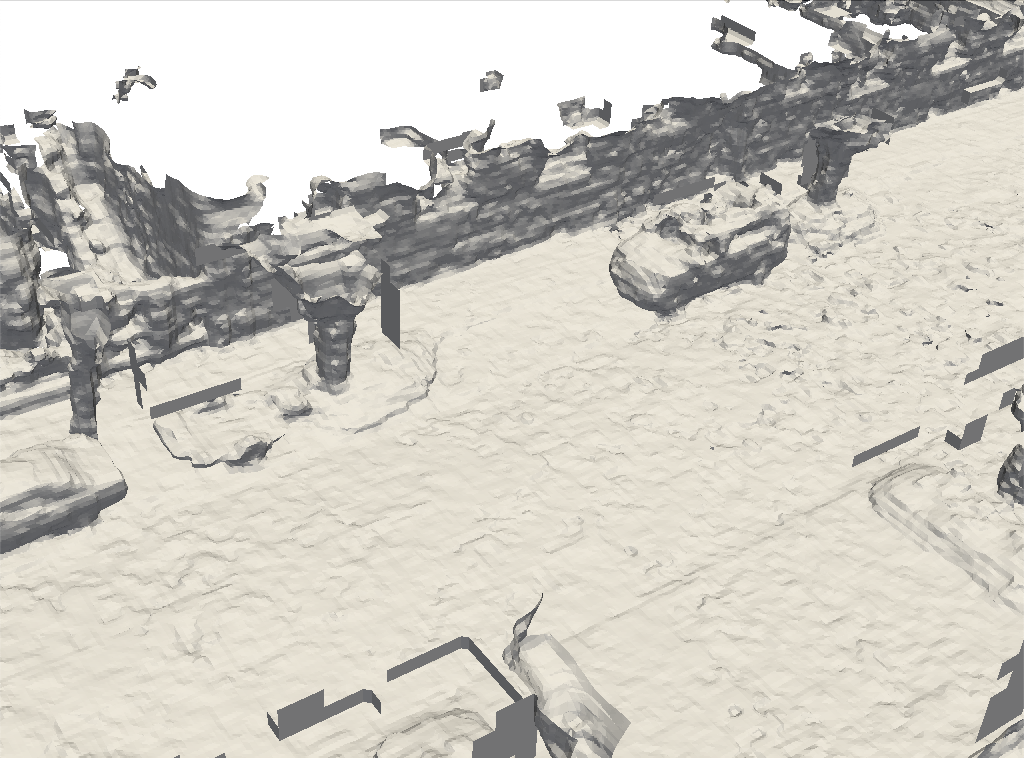
\includegraphics[width=1\linewidth]{figures/kitti_3_shine.png}
        \caption*{(c)SHINE-Mapping}
	\end{minipage}\hfill
    \begin{minipage}{0.5\linewidth}
		\centering
		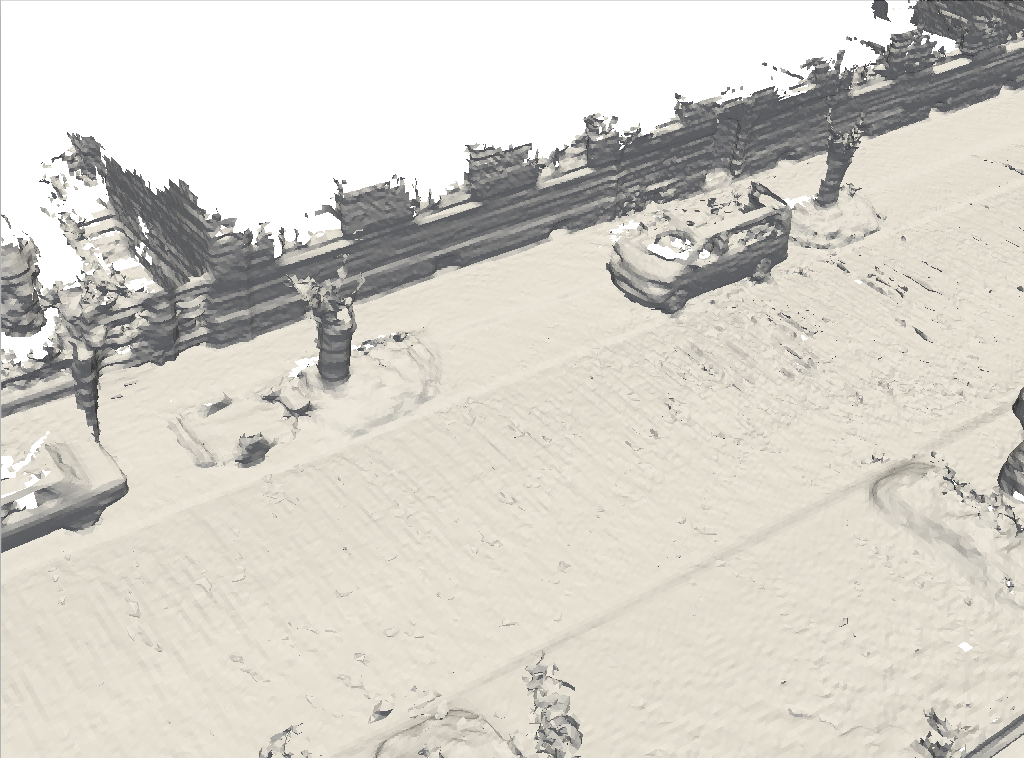
\includegraphics[width=1\linewidth]{figures/kitti_3_vdb.png}
        \caption*{(d)VDB Fusion}
	\end{minipage}
\end{figure}

\begin{figure}[htbp]
    \centering
    \begin{minipage}{0.5\linewidth}
    \centering
    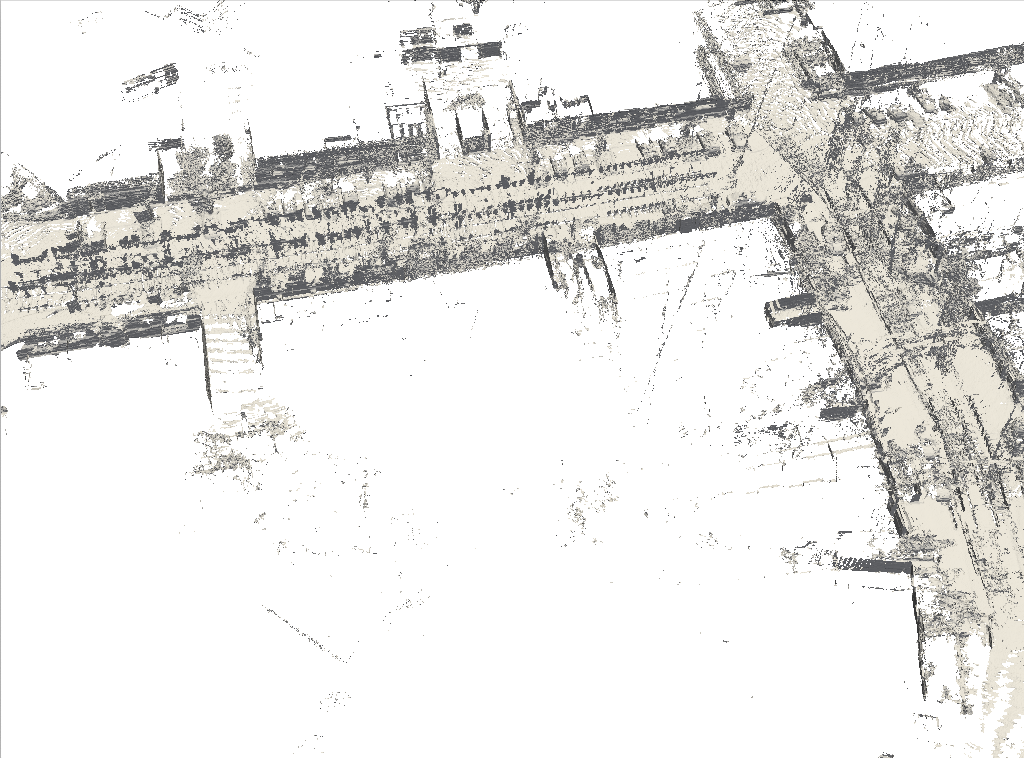
\includegraphics[width=1\linewidth]{figures/kitti_1_voxblox.png}
    \end{minipage}\hfill
    \begin{minipage}{0.5\linewidth}
    \centering
    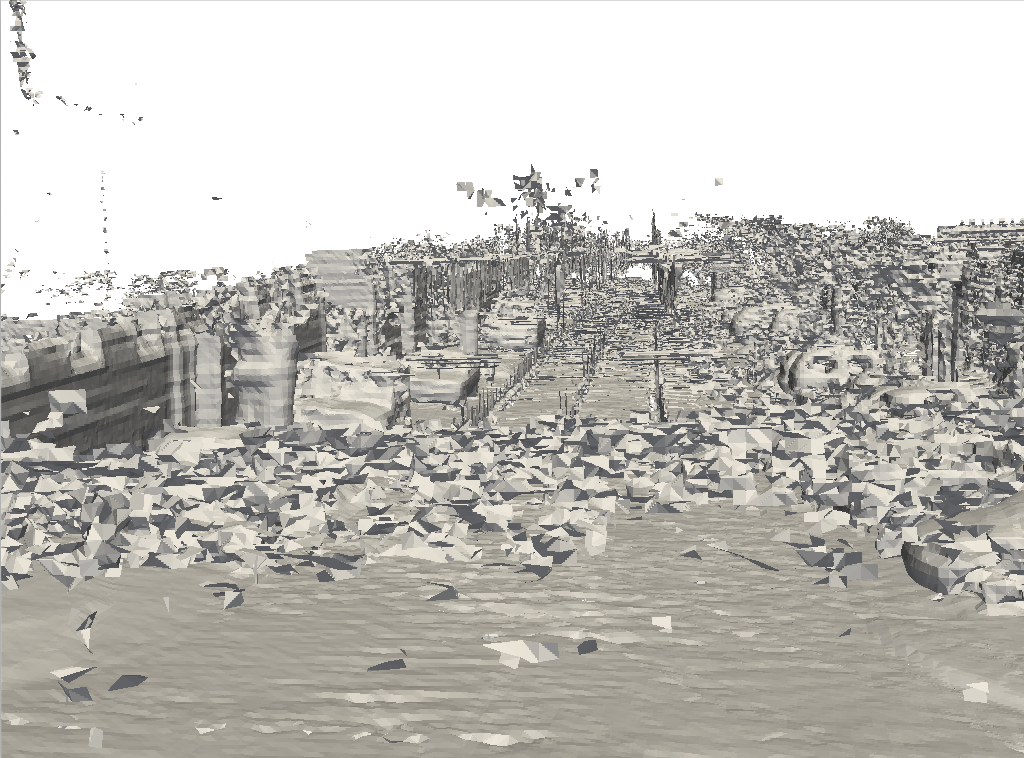
\includegraphics[width=1\linewidth]{figures/kitti_2_voxblox.png}
    \end{minipage}
    \vfill
    \begin{minipage}{0.5\linewidth}
    \centering
    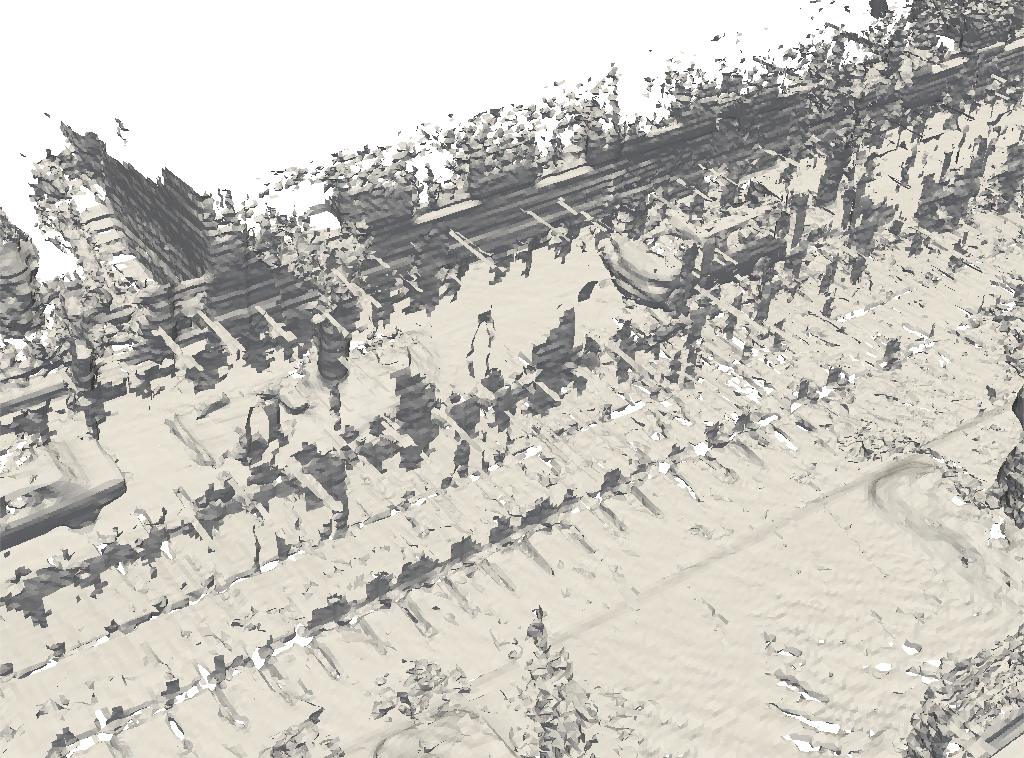
\includegraphics[width=1\linewidth]{figures/kitti_3_voxblox.png}
    \end{minipage}\caption*{(e)Voxblox}
    \caption{5种不同方法在KITTI数据集Seq00序列上的结果。}\label{kittiresult}
\end{figure}
同样的,本文使用3种基于神经隐式表达的建图方法在New College数据集的Seq01序列上进行了实验实验结果如图\ref{ncdresult}所示。在具有更多噪声的场景中建图是具有挑战性的,所有方法的效果均低于在合成场景与相对噪声较小的真实场景。由于该数据集拥有网格地图的真实数据,本文对其几何建图精度进行了评估,结果如表\ref{ncdmetric}所示。由于噪声较大,该评估将阈值$threshold$设置为20cm。本文算法在几何精度指标上与SHINE-Mapping相近,效果远优于Vox-Fusion。
\begin{figure}[htbp]
    \centering
\begin{minipage}{0.5\linewidth}
    \centering
    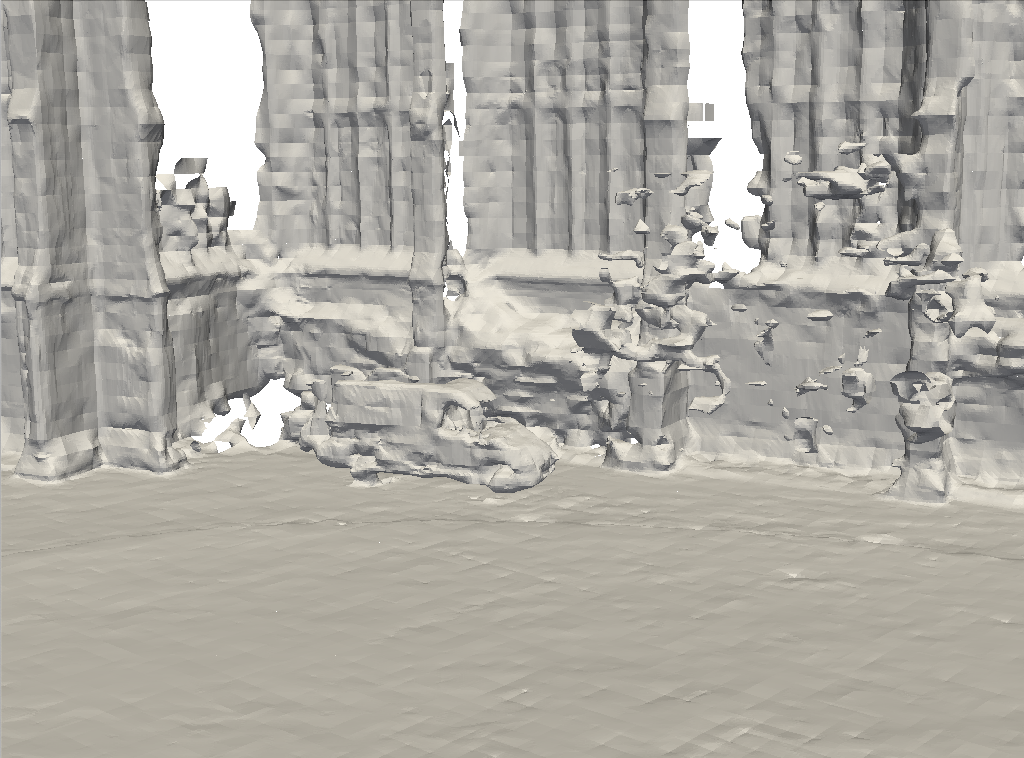
\includegraphics[width=1\linewidth]{figures/ncd_1_vox.png}
\end{minipage}\hfill
\begin{minipage}{0.5\linewidth}
    \centering
    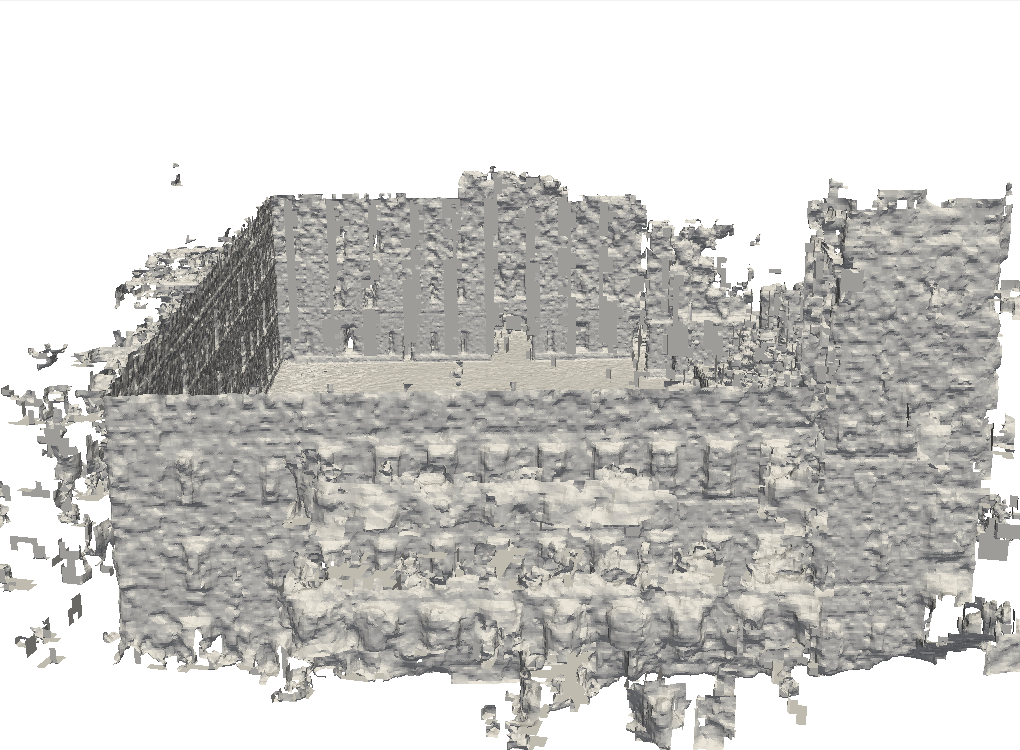
\includegraphics[width=1\linewidth]{figures/ncd_1_shine.png}
\end{minipage}
\vfill
\begin{minipage}{0.5\linewidth}
    \centering
    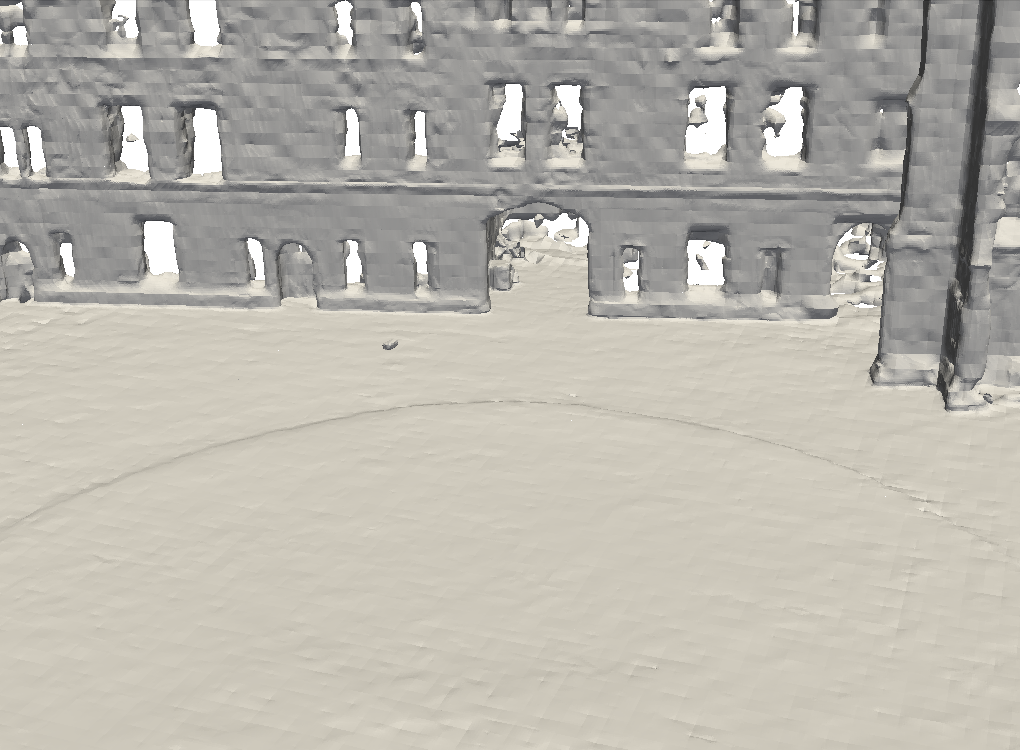
\includegraphics[width=1\linewidth]{figures/ncd_2_vox.png}
\end{minipage}\hfill
\begin{minipage}{0.5\linewidth}
    \centering
    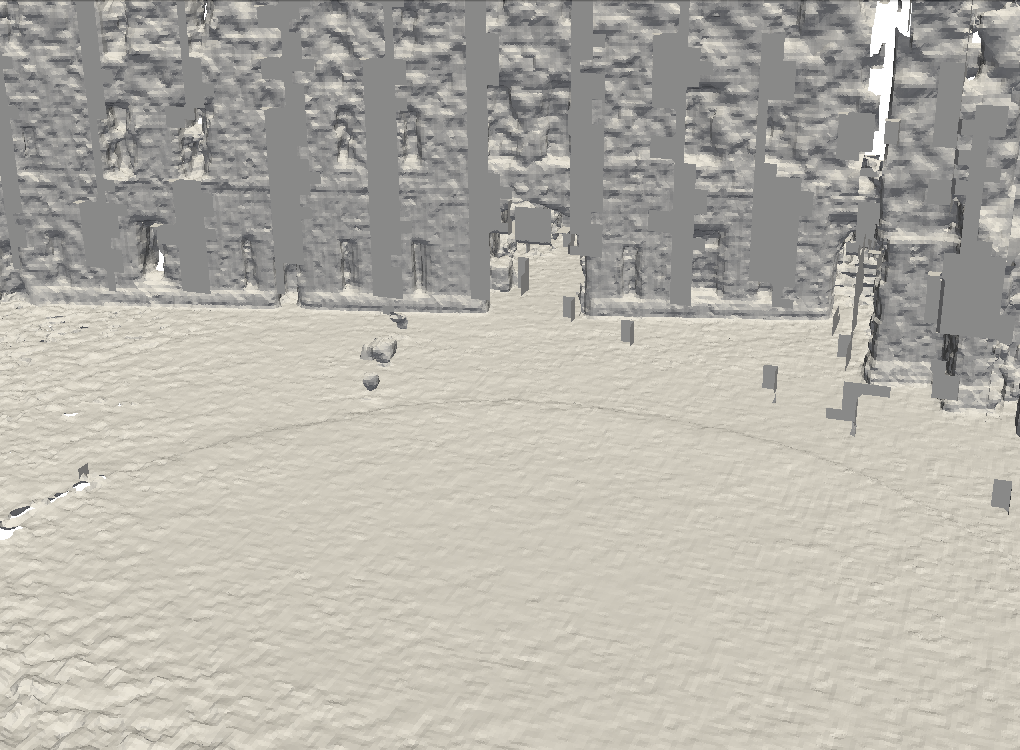
\includegraphics[width=1\linewidth]{figures/ncd_2_shine.png}
\end{minipage}
\vfill
\begin{minipage}{0.5\linewidth}
    \centering
    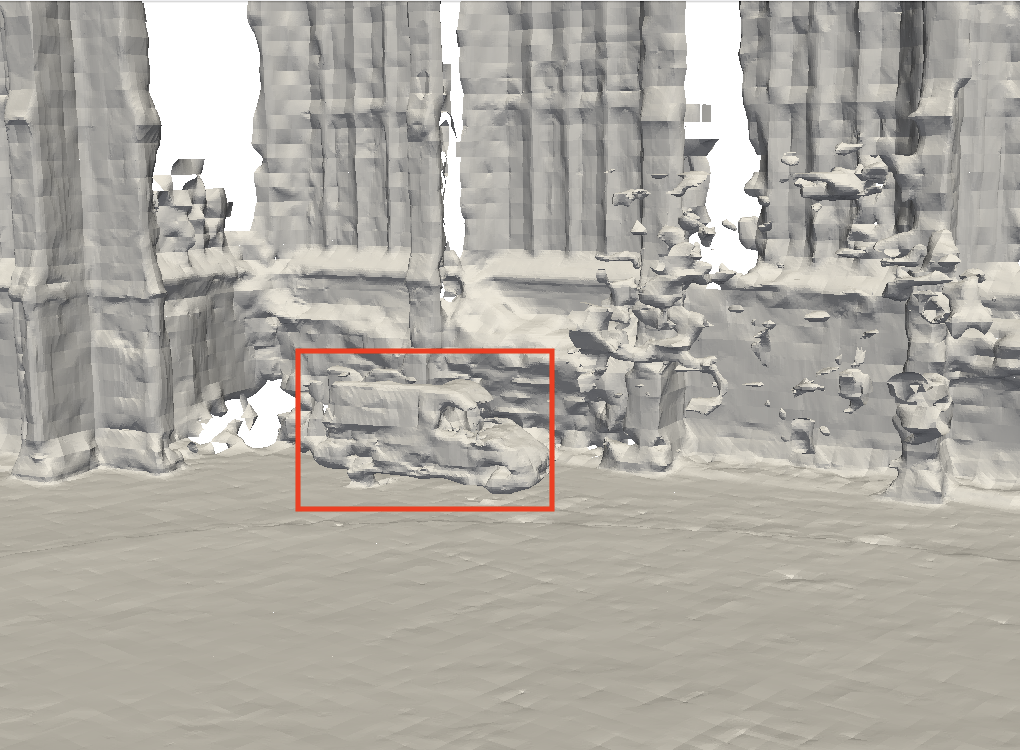
\includegraphics[width=1\linewidth]{figures/ncd_3_vox.png}
    \caption*{(a)Ours}
\end{minipage}\hfill
\begin{minipage}{0.5\linewidth}
    \centering
    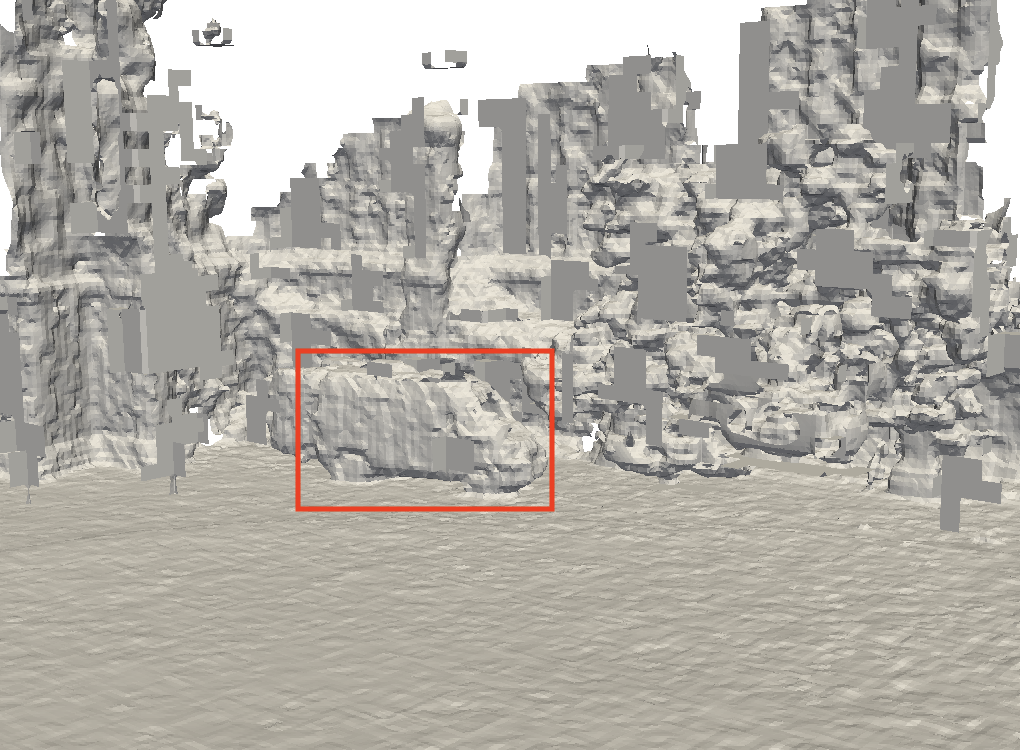
\includegraphics[width=1\linewidth]{figures/ncd_3_shine.png}
    \caption*{(b)Vox-Fusion}
\end{minipage}
\end{figure}

\begin{figure}[htbp]
    \centering
    \begin{minipage}{0.5\linewidth}
    \centering
    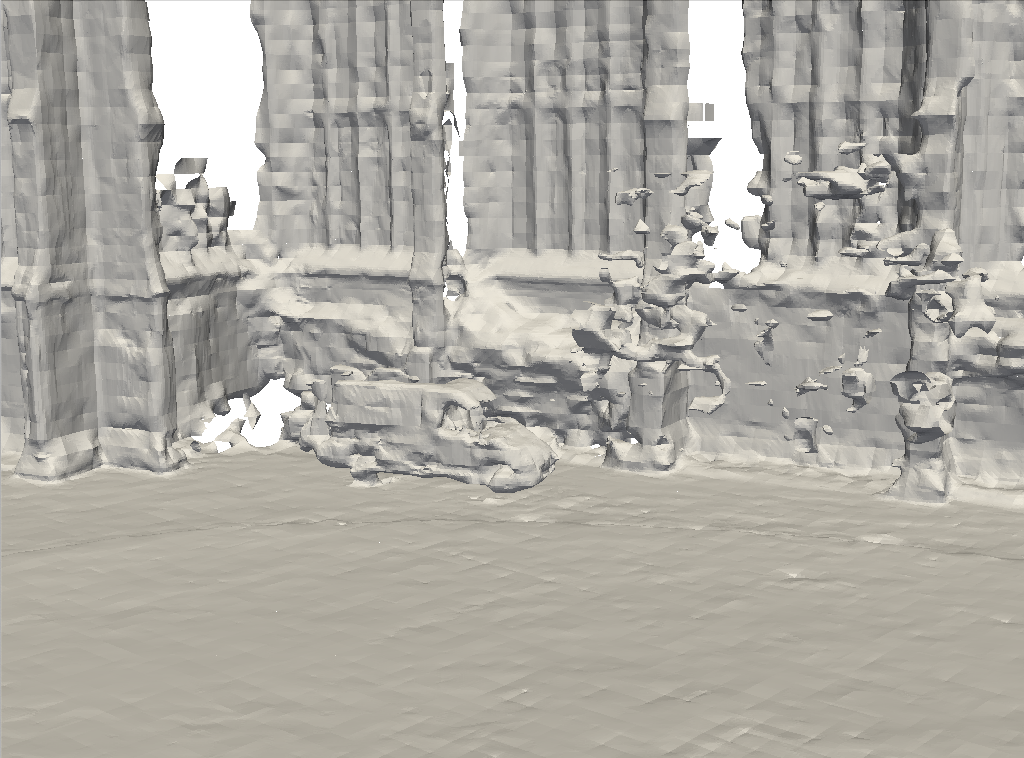
\includegraphics[width=1\linewidth]{figures/ncd_1_vox.png}
    \end{minipage}\hfill
    \begin{minipage}{0.5\linewidth}
    \centering
    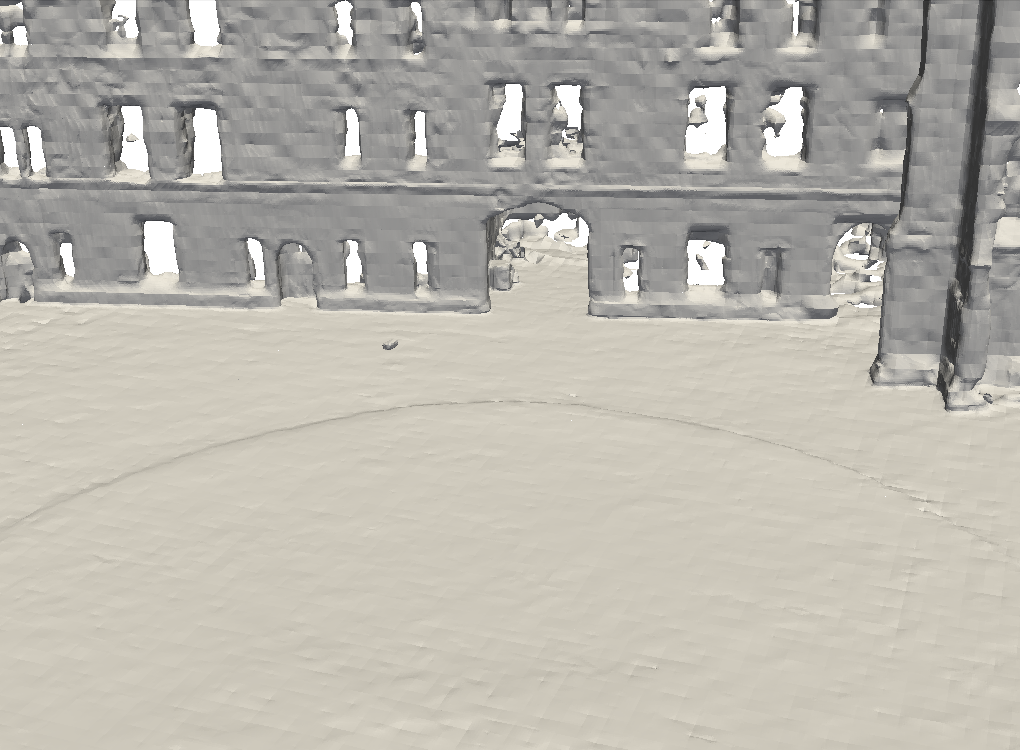
\includegraphics[width=1\linewidth]{figures/ncd_2_vox.png}
    \end{minipage}
    \vfill
    \begin{minipage}{0.5\linewidth}
        \centering
        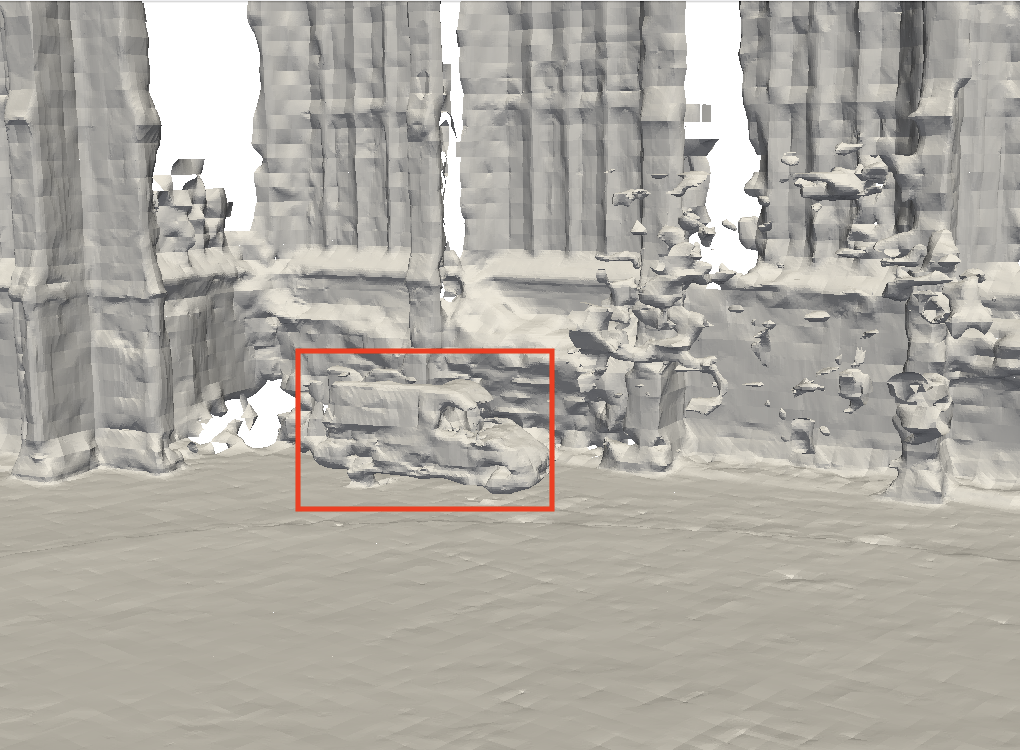
\includegraphics[width=1\linewidth]{figures/ncd_3_vox.png}
        \end{minipage}
    \caption{3种基于神经网络的隐式建图方法在New College数据集上的结果。}\label{ncdresult}
\end{figure}

\begin{table}[htbp]
    \centering
    \caption{定性测量的不同方法在New College数据集上建图的几何精度,将目标地图与重建地图之间对应点重合的阈值$threshold$设置为20cm。}\label{ncdmetric}
    \begin{tabular}[htbp]{llccccc}
        \toprule
        \multicolumn{2}{l}{方法} & $\mathbf{Comp.}$(cm) & $\mathbf{Acc.}(\%)$ & $\mathbf{C-l1}$(cm) &  $\mathbf{Comp. Ratio}$(\%) &$\mathbf{F1-score}$\\
        \midrule
        \multicolumn{2}{l}{Voxblox} & 14.9 & 90.6 &12.1 &87.8&87.9\\
        \multicolumn{2}{l}{VDB Fusion} & 12.0&92.1&9.4&91.3&92.6 \\
        \multicolumn{2}{l}{SHINE-Mapping} & 10.0&93.5&8.4&93.6&93.7 \\
        \multicolumn{2}{l}{Vox-Fusion} & 14.2 & 89.7& 13.6&89.4&89.0\\
        \midrule
        \multicolumn{2}{l}{Ours+bce} &10.3& 93.2 & 7.9 &93.5&91.3\\
        \bottomrule
    \end{tabular}
\end{table}
本文在KITTI数据集上进行了语义建图精度评估实验。如表\ref{kittimetrics}所示,在KITTI数据集的8个序列上,本文对每个关键帧采样1000个点云,使用训练完成的模型与解码器进行推理得到采样点的语义标签,并与SemanticKITTI数据集的语义标签进行比较以计算语义建图精度。结果显示在室外大规模场景下,本文语义建图方法可以达到约90\%的准确率。将预测出的语义标签映射为不同颜色后的效果如图\ref{semresult}所示。

\begin{table}[htbp]
    \centering
    \caption{本文方法在KITTI数据集上的语义建图精度评估。}\label{kittimetrics}
    \begin{tabular}[htbp]{cccccccccc}
        \toprule
        \multicolumn{2}{l}{指标} & Seq00 & Seq01 & Seq02 &Seq03&Seq04&Seq05&Seq06&Seq07 \\
        \midrule
        \multicolumn{2}{l}{AUC\%} & 91.4 & 92.0 & 89.7 & 90.6 &87.6&88.7&91.2&92.5\\
        \multicolumn{2}{c}{IoU\%} & 83.2& 84.3&79.8&86.2&75.4&77.8&87.3&87.1 \\
        \bottomrule
    \end{tabular}
\end{table}
\begin{figure}[htbp]
	\centering
	\begin{minipage}{1\linewidth}
		\centering
		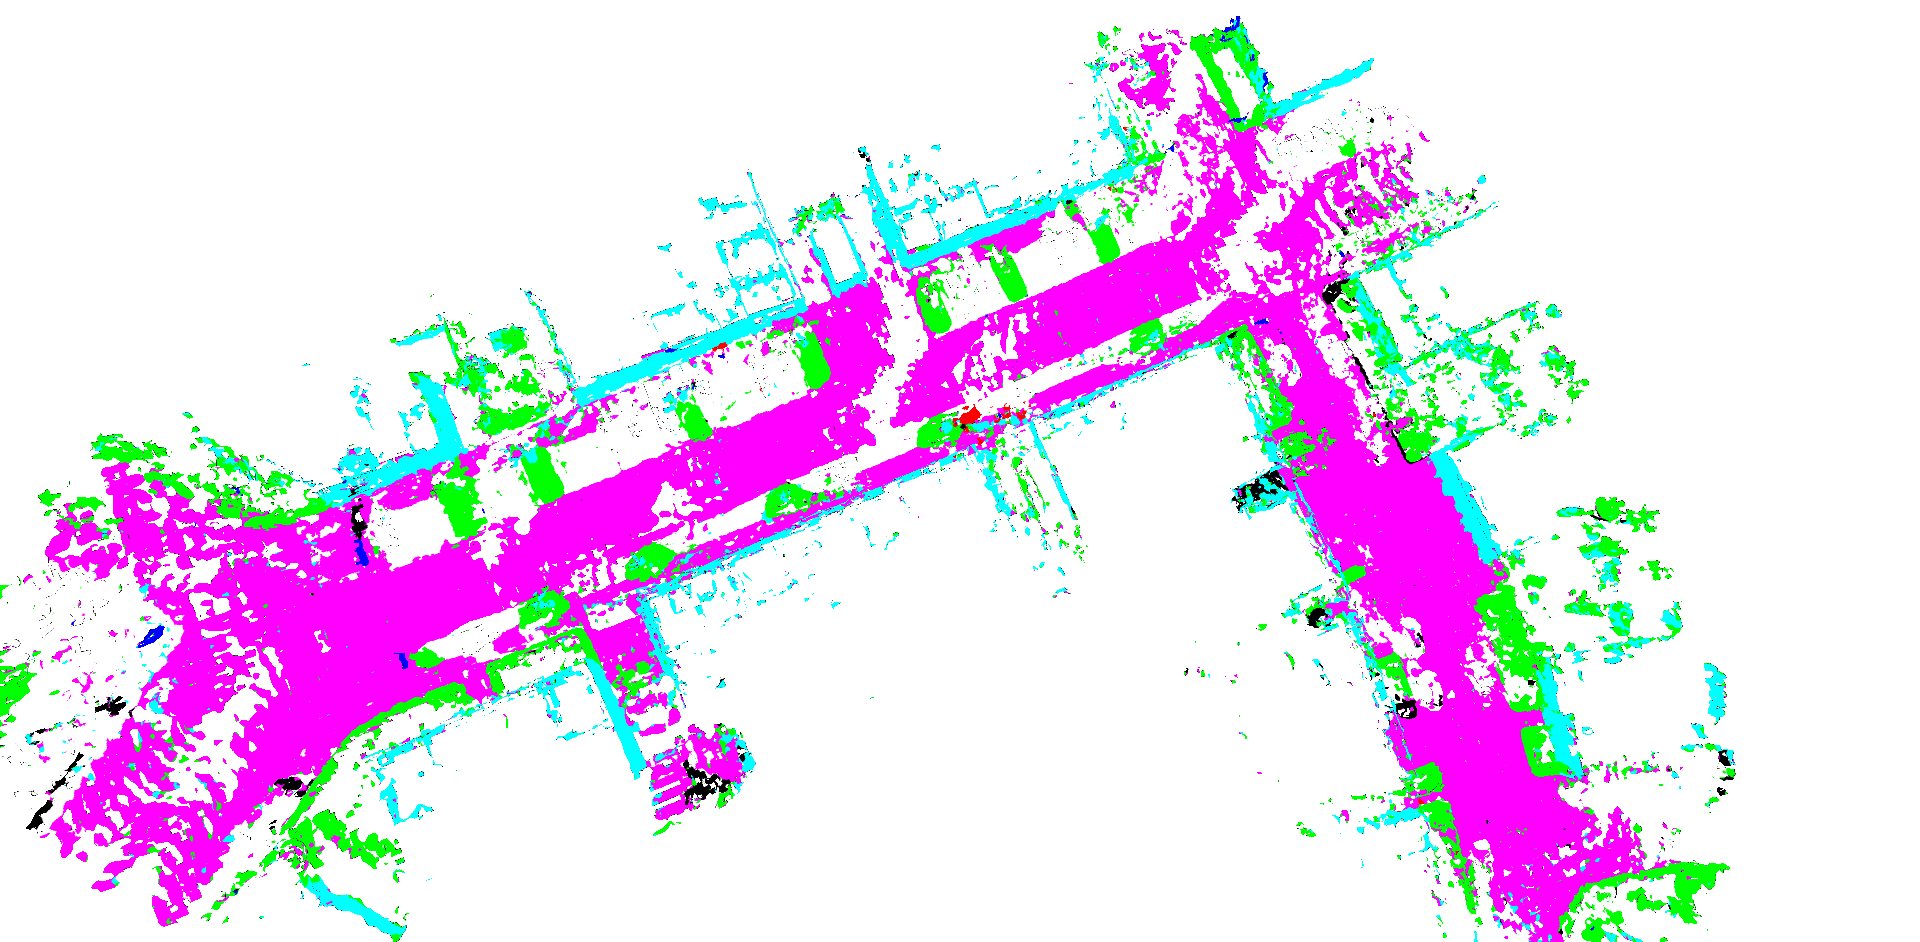
\includegraphics[width=1\linewidth]{figures/sem1.png}
	\end{minipage}
    \vfill
	\begin{minipage}{1\linewidth}
		\centering
		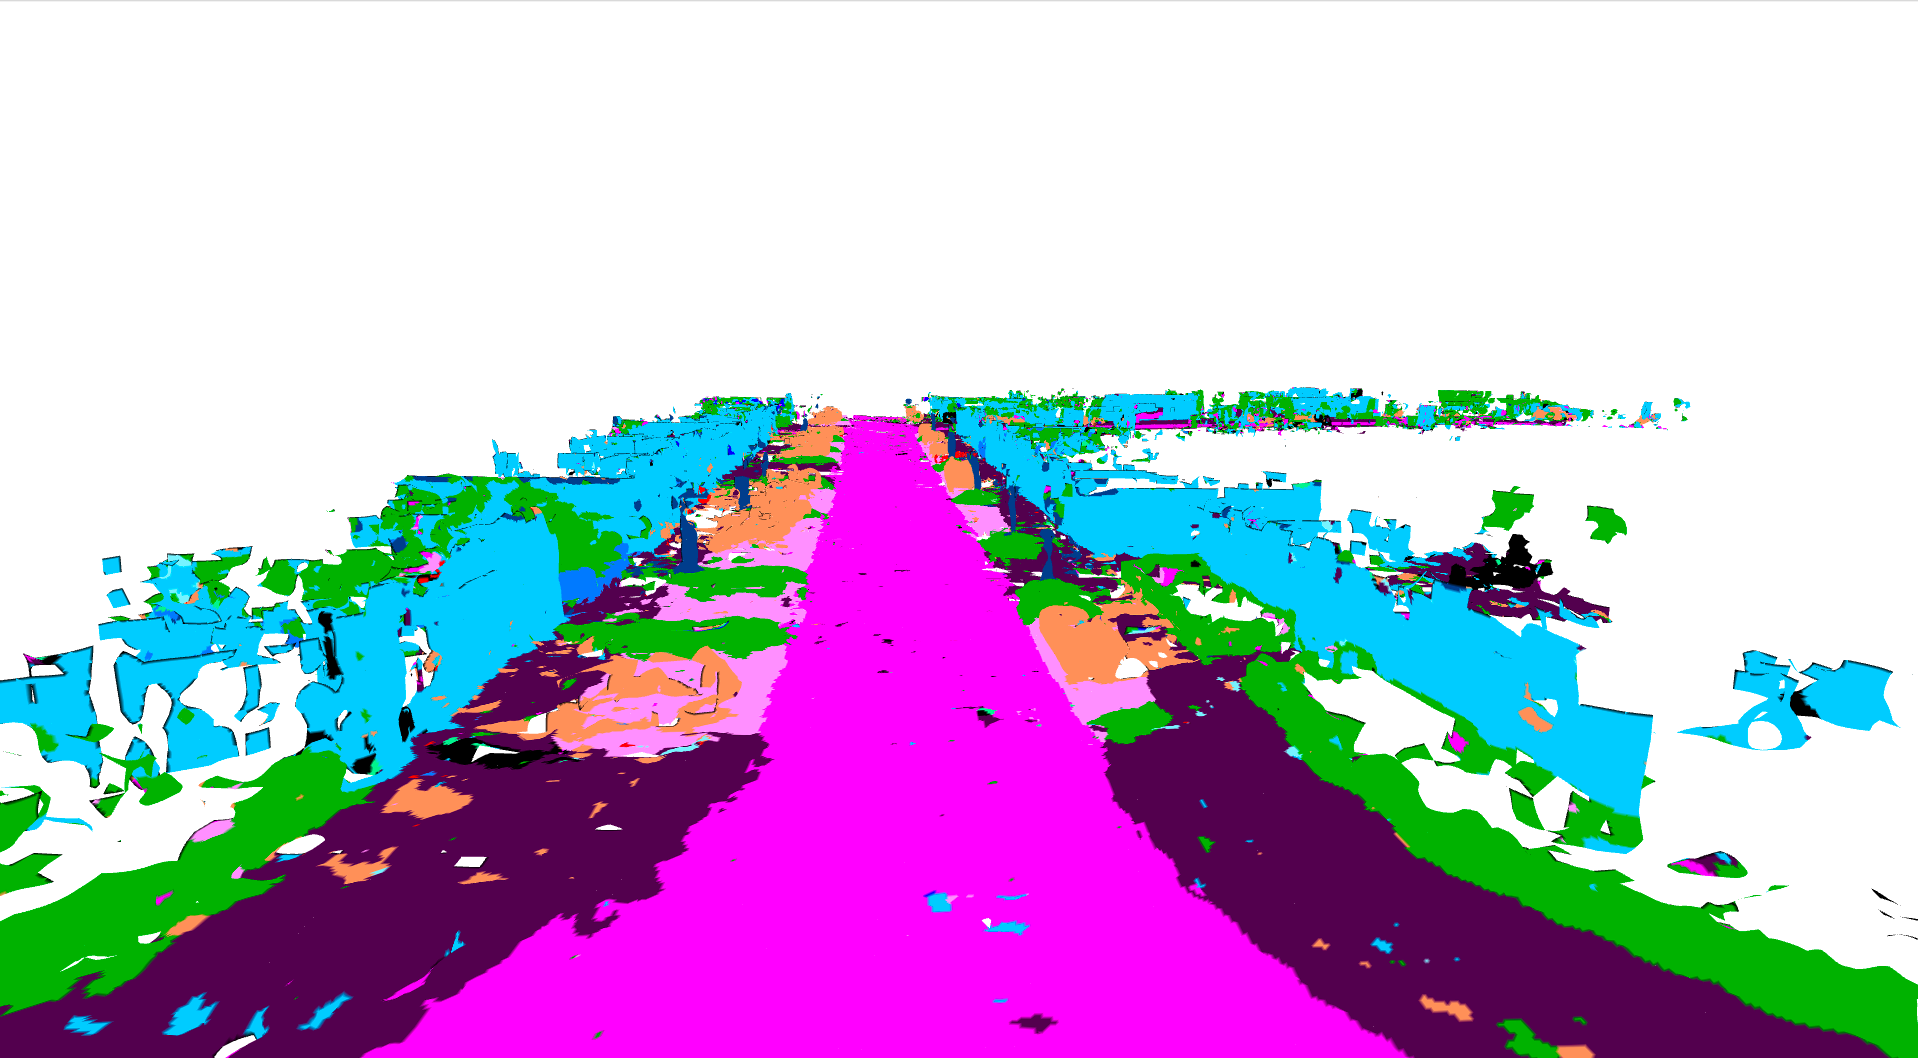
\includegraphics[width=1\linewidth]{figures/sem2.png}
	\end{minipage}
    \caption{在KITTI数据集上进行语义建图后,使用模型预测每一顶点的语义标签并将其映射为不同颜色。}\label{semresult}
\end{figure}

\subsection{算法时间与内存占用}
为了加速本文方法,除了使用多线程并行实现增量建图与全局建图外,本文测量了渲染和训练过程中关键步骤的耗时,如体素分配,求交运算和体渲染等步骤,并进行了分析。本文实验在单张Nvidia RTX 3090显卡上进行,结果列于表\ref{times}中。可以看出使用C++实现的体素相关操作运行速度较快,在系统运行中耗时占比远小于其他操作。在采样1024条光线的情况下,本文系统中单次建图迭代需要40-50ms。设置每次建图过程中迭代10-50次,本文系统最快可以达到2Hz的建图速度。
\begin{table}[htbp]
    \centering
    \caption{系统中关键步骤平均耗时。}\label{times}
    \begin{tabular}[htbp]{llc}
        \toprule
        \multicolumn{2}{l}{步骤} & 时间\\
        \midrule
        \multicolumn{2}{l}{增量建图} & 50ms\\
        \multicolumn{2}{l}{全局建图} & 50ms \\
        \midrule
        \multicolumn{2}{l}{体素分配} & 0.1ms \\
        \multicolumn{2}{l}{光线体素求交} & 0.9ms \\
        \multicolumn{2}{l}{体渲染} & 4ms \\
        \multicolumn{2}{l}{参数优化} & 6ms \\
        \bottomrule
    \end{tabular}
\end{table}

相较于同样使用基于体素的八叉树的SHING-Mapping方法,本文方法的内存消耗与其几乎相同。但NICE-SLAM方法使用4个网格地图并需要在系统启动前分配所有地图空间,与之相比本文方法在内存消耗上占据优势。详细结果如图\ref{memory}所示,本文方法可以在显著使用更少内存的同时实现更精细的建模。
\begin{table}[htbp]
    \centering
    \caption{不同方法在Mai City数据集01序列上建图的理论内存消耗。由于NICE-SLAM使用了4个特征网格,每一个特征网格对地图所有区域分配内存,因此内存消耗巨大。本文方法只使用一个特征网格,且只对观察到的地图区域分配体素与特征,使用较小的内存可以达到精细度更高的建图效果。}\label{memory}
    \begin{tabular}[htbp]{llcc}
        \toprule
        \multicolumn{2}{l}{方法} &解码器 & 地图特征\\
        \midrule
        \multicolumn{2}{l}{SHINE-Mapping} & 0.56MB & 7.09MB\\
        \multicolumn{2}{l}{NICE-SLAM} & 0.22MB & 560MB\\
        \midrule
        \multicolumn{2}{l}{Ours} & 1.04MB & 7.09MB\\
        \bottomrule
    \end{tabular}
\end{table}

